\documentclass[11pt,letterpaper,fleqn]{report}
\usepackage{amsmath,amsthm,amsfonts,amssymb,amscd}
\usepackage{fullpage}
\usepackage{lastpage}
\usepackage{enumerate}
\usepackage{fancyhdr}
\usepackage[percent]{overpic}
\usepackage{mathrsfs}
\usepackage{wrapfig}
\usepackage{multirow}
\usepackage{amsmath}
\usepackage{amssymb}
\usepackage{amscd}
\usepackage{lscape}
\usepackage{graphicx}
\usepackage[usenames,dvipsnames]{color}
\usepackage{listings}
\usepackage[usenames,dvipsnames,svgnames,table]{xcolor}
\usepackage[left=2.5cm,right=2.5cm,top=2.5cm,bottom=2.5cm, headsep = 0.9cm]{geometry}
\usepackage{verbdef}
\setlength{\parindent}{0.0in}
\setlength{\parskip}{0.0in}
\usepackage{setspace}
\definecolor{gray}{RGB}{90,90,90}
\usepackage[colorlinks=true, linktoc=all, linkcolor=blue]{hyperref}
\newcommand\hwnum{8}
\newcommand\yourname{\large Andrew J. Spieker}
\newenvironment{answer}[1]{
  \subsubsection*{\large Problem #1.}
}

\pagestyle{plain}

\begin{document}
\centerline{\textbf{\Large{An Introduction to R}}}
\centerline{\textbf{Authors: Andrew J. Spieker and Brian D. Williamson}}
\tableofcontents

\chapter{Introduction}
This document is meant for students to get an introductory look at R (and how it compares to and differs from STATA), and to facilitate a transition for both students and instructors from STATA to R, using both the base R functions and the \texttt{uwIntroStats} package developed by Scott S. Emerson, M.D. Ph.D., Andrew J. Spieker, and Brian D. Williamson in the University of Washington Department of Biostatistics.\\

R is a functional language at the basic level, meaning that even the simple expression \texttt{3 + 5} is handed to a function called \texttt{evaluate()}, which then returns the result. Most objects and functions have a print function, so we can either print and display results or store them as an object. STATA, on the other hand, is a command style language. The user types in a command and the result is displayed. In this file we will present some of the useful R functions, but there are many more that we leave to the reader to go out and find. Also, even if we do present a function here, we will be doing so at the most basic level. Many of the functions have more capabilities than what we show.

\chapter{Project Management}
\section{The Workspace}
There are a few differences between R and STATA when it comes to data and project management. The first concept that we must cover is that of the workspace. In STATA, you are only allowed to read in one data set at a time. This data set is your entire workspace, and thus all functions and calls manipulate the data set. In R, however, the workspace consists of many different data sets, values, and functions. Any variable that is assigned a name becomes part of the workspace. Upon exit from R, the program asks the user if they wish to save the workspace. Saying yes saves all variables, functions, and data sets and then loads them back in to the workspace upon startup of the program the next time. It is generally good practice to save the workspace, especially if you know that you will continue to work with the same data next time.

To start, we will assume you are running R from the command line. Later on, if you wish, we will introduce a convenient graphical user interface. However, it is good to learn the basics from the command line and know what is happening behind the buttons in the GUI. Once you navigate to the correct directory for R (in a Windows machine this is generally in ``C:\textbackslash Program Files\textbackslash R\textbackslash R-version\textbackslash bin'' - substitue the version of R you downloaded for ``version''), you simply type ``R'' and the program will start, displaying a screen similar to this:

\begin{figure}[h!]
\centering
	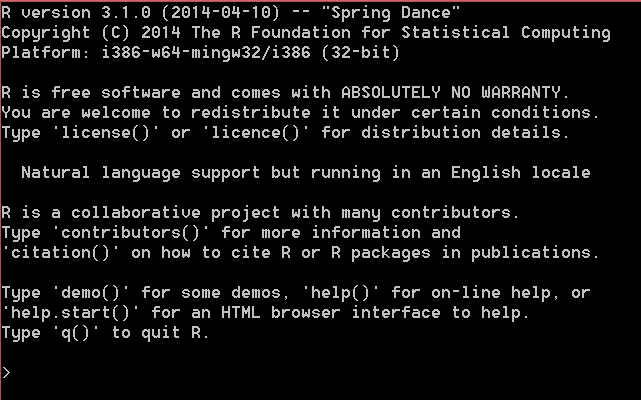
\includegraphics[width=5in]{r_welcome.png}
\end{figure}

If you type `q()', you are prompted to \texttt{Save workspace image? [y/n/c]: }, where `\texttt{y}' is yes, `\texttt{n}' is no, and `\texttt{c}' is cancel. If you type `\texttt{y}', then two files are created: a \texttt{.Rhistory} file and a \texttt{.RData} file. You can load the \texttt{.RData} file at the beginning of a session with the \texttt{load()} function, and it brings in all of your variables, data sets, and functions. The \texttt{.Rhistory} file saves all of your commands from the session. If you are working with a few different projects, it is a good idea to have a workspace for each of these projects. Then any one workspace doesn't get too cluttered.
\section{Scripts}
Scripts are useful files that can be run by R. A script file can be created in any directory on your computer. Then it can be ``sourced'', using the \texttt{source()} function (given the file path) to run all of the functions saved in the script file. A script is a useful place to write all of your function calls so that you can save them for later. For example, on a Windows computer, we could create a script file on the Desktop by using any text editor (Notepad or any other that you prefer) and saving the file with the \texttt{.R} extension, such as:
\begin{verbatim}
test_script.R
\end{verbatim}
We can then load all of the functions and run all of the code saved in the script by opening R and typing (recall that our script file is located on the desktop)
\begin{verbatim}
source(``C://Users//Brian Williamson//Desktop//test_script.R'')
\end{verbatim}
\section{Comments}
Commenting your files is always a good idea. Comments provide information as to why you are using certain functions at certain times. The comment key in R is \texttt{\#}. If you type this at any point on a line, the rest of the line will not be run by R.

\chapter{Data}

\section{Data Types (`storage.mode')}
A huge reason for using R at all is its data capabilities. There are many types of data in R, and thus it is important to know what kind of data you are dealing with at a given time. The ``\texttt{storage.mode()}'' function returns what type the data is. The basic data types are:

\subsection{Numeric}
Decimal values are numerics. Numeric is the default computational data type in R. \emph{Note for the curious: all real numbers in R are stored as ``doubles'', meaning that the IEEE floating point number is stored as a 64 bit word rather than a 32 bit word.} There are two subtypes of numeric values. Most of the time there is no need to worry about the difference between them, but every once in a while you need to know which type you are dealing with.\\

\textbf{Integer}\\
A whole number. \\
\newline \textbf{Double}\\
A real number (whole number plus fractional part).\\

\subsection{Character}
A character is an object which represents string values. For example, "3" is a character. To convert an object into a character, use the \texttt{as.character()} function. 

\subsection{Logical}
\texttt{TRUE} and \texttt{FALSE} are the logical values in R, usually produced by comparisons. The standard logical operators in R are: 
\begin{tabular}{ll}
``\&"  & and \\
``$\mid$" & or \\
``!" & negation\\
``==" & equals
\end{tabular}

\subsection{NA, NULL, Inf, and NaN}
\texttt{NA} denotes a missing value in R. \texttt{NA} is a logical constant of length 1.\\

\texttt{NULL} is the null object in R. Functions and expressions whose values are undefined sometimes return \texttt{NULL}. If a \texttt{NULL} value is compared to another (for example, \texttt{NULL == 0}), then the result will be the expression \texttt{logical(0)}. The length of the \texttt{NULL} object is 0.\\
\texttt{Inf} is returned by dividing any number besides 0 by 0.\\
\texttt{NaN} (not a number) is returned by the expression dividing 0 by 0.\\

\begin{verbatim}
0/0
[1] NaN
1/0
[1] Inf
\end{verbatim}

\subsection{Factor}
A factor stores the nominal values of the data (starting with 1) in a vector, and stores the associated names of the data as a vector of character strings. A factor is created with the \texttt{factor()} function. For example, let's say that we have a vector with twenty \texttt{``male''}'s and twenty \texttt{``female''}'s. Then a factor would store this data as twenty 1s and twenty 2s, and would have a key telling us that \texttt{1} was male and \texttt{2} was female. \emph{For the really curious: factors are really data structures, since they are a vector with attributes.}
%\subsubsection{Complex}
%A complex number - has an imaginary component.

\section{Data Structures}
There are a variety of data structures in R. They include vectors, matrices, arrays, data frames, lists, and factors.

\subsection{Vectors}
A vector is the most simple data structure in R. A vector stores any number of individual values, but they must be all of the same type. A vector is created with the \texttt{c()} function.

\subsection{Matrices}
A matrix is a table, is essentially a two-dimensional vector. All values in the matrix must be of the same data type, and a matrix must be rectangular - that is, each row must have the same number of columns as the others and each column must have the same number of rows as the others. A matrix is created with the \texttt{matrix()} function. 

\subsection{Arrays}
An array is a high-dimensional matrix. An array is created with the \texttt{array} function.

\subsection{Data frame}
A data frame is a table, like a matrix. However, the columns in a data frame may have different data types. A data frame is created with the \texttt{data.frame()} function.

\subsection{List}
A list is an ordered collection of objects. The values in a list can be any data type or data structure, and they don't have to have the same size. A list is created with the \texttt{list()} function. \emph{A note for the curious: lists indirectly reference their values. They are stored in different places in memory as addresses.} Lists are sometimes returned from functions.

\section{Assigning a Value to a Variable}
Let's say we want to creat a variable called \texttt{junk}. Then we must assign \texttt{junk} a value. Here we will assign it the number \texttt{1}. Thus, we type 
\begin{verbatim}
junk <- 1
\end{verbatim}
And now any time that we wish to see what \texttt{junk} is, we type \texttt{junk} and get the output 
\begin{verbatim}
junk
[1] 1
\end{verbatim}
Any time we wish to assign a value to a variable, we use the ``\texttt{<-}'' function. This guarantees that we perform the correct assignment (some functions and packages were developed in a time where using ``='' as assignment will not work correctly).

\section{Returning a Value from a Data Structure}
There are three main ways of accessing data in a data set. The main ways deal with data sets in vector or matrix form (similar syntax), list form, or data frame form. 

\subsection{The ``[ ]'' Operator}
The first way we will cover is for vectors and matrices. Let's say we have a vector representing the numbers 1-10. This vector can be stored as \begin{verbatim}> test <- c(1,2,3,4,5,6,7,8,9,10) \end{verbatim} Now if we wish to access the 6, we type 
\begin{verbatim}
test[6] 
\end{verbatim}
Which returns
\begin{verbatim}
[1] 6
\end{verbatim} 
Recall that R is a functional language at its base. Thus, if we want to see the sixth value of \texttt{test}, we can type in any expression which will evaluate to 6. For example:
\begin{verbatim}
test[3+3]
[1] 6
\end{verbatim}
Now, a vector is simply a matrix with one row. Thus let's consider a matrix with 735 rows and 30 columns (we will be using this matrix later as well) called \texttt{mri}. If we wish to access an entry in the matrix we type in the row and column of interest: 
\begin{verbatim}
mri[1,1]
[1] 1
\end{verbatim}
Which returns the value in row 1, column 1 as we requested.

\subsection{The ``\$'' Operator}
A data frame, as we discussed earlier, is a list of vectors. Let's use the \texttt{mriTest} data frame that we created earlier. Now we can access a value from the data frame either by the \texttt{[rownum,colnum]} or \texttt{[rownum,"colname"]} function or by the \texttt{\$colname[rownum]} function:
\begin{verbatim}
mriTest[1,1]
[1] 1 
mriTest[1,"ptid"]
[1] 1 
mriTest$ptid[1]
[1] 1 
\end{verbatim}

\section{Indexing Values in a Data Structure}
Sometimes, it is useful to access more than one value from a data structure. 

\subsection{The ``[ ]'' operator}
If we want to see the first five elements of the vector, we type
\begin{verbatim}
test[1:5]
\end{verbatim}
which returns
\begin{verbatim}
[1] 1 2 3 4 5 
\end{verbatim}
Now recall the \texttt{mri} data set. If we wish to access the entire first row (a vector!) we type 
\begin{verbatim}
mri[1,]
\end{verbatim}
Which means that we are selecting the first row and all of the columns. The \texttt{[row,column]} format is followed for matrices. The output of this call is 
\begin{verbatim}
  ptid mridate age male race weight height packyrs yrsquit alcoh physact chf chd
1    1  120791  72    1    2    173    169      54       0     0    9.84   0   1
  stroke diabetes genhlth ldl alb crt plt sbp    aai   fev dsst atrophy whgrd
1      2        0       3 135 3.7 1.4 275 139 1.0303 1.284   25      20     2
  numinf volinf obstime death
1      1 7.4613    2110     0
\end{verbatim}

\subsection{Special Issues for Indexing a Matrix}
However, when we are subscripting a matrix, we may wish to be sure what class our returned value is. For example, a test matrix
\begin{verbatim}
m <- matrix(rep(1, 30), nrow=3)
m
     [,1] [,2] [,3] [,4] [,5] [,6] [,7] [,8] [,9] [,10]
[1,]    1    1    1    1    1    1    1    1    1     1
[2,]    1    1    1    1    1    1    1    1    1     1
[3,]    1    1    1    1    1    1    1    1    1     1
\end{verbatim}
If we want the first row of the matrix, and want it to be a matrix, we will run into problems if we simply type \texttt{m[1,]}. 
\begin{verbatim}
m[1,]
 [1] 1 1 1 1 1 1 1 1 1 1
\end{verbatim}
Notice that this returned a vector! If we want a matrix, we must type
\begin{verbatim}
m[1,,drop=FALSE]
     [,1] [,2] [,3] [,4] [,5] [,6] [,7] [,8] [,9] [,10]
[1,]    1    1    1    1    1    1    1    1    1     1
\end{verbatim}
Adding the \texttt{drop=FALSE} argument after our row and column specifications told R not to drop dimensions and create a vector.
\subsection{The ``\$'' Operator}
Let's use the \texttt{mriTest} data frame that we created earlier. Now we can access a column of the data frame either by the \texttt{[,colnum]} or \texttt{[,"colname"]} function or by the \texttt{\$colname} function, as we see here (we only get the first three rows to save paper):
\begin{verbatim}
mriTest[1:3,1]
[1] 1 2 3
mriTest[1:3,"ptid"]
[1] 1 2 3
mriTest$ptid[1:3]
[1] 1 2 3
\end{verbatim}
Last, variables in matrices, lists, and data frames can both be accessed using the \texttt{\$} operator. Create \texttt{sampleList} to have a vector of strings, a matrix, and a single number as follows:
\begin{verbatim}
sampleList <- list(c("One", "Two", "Three"), mri, 1)
\end{verbatim}
Now we wish to name the elements of \texttt{sampleList}:
\begin{verbatim}
names(sampleList) <- c("strings", "matrix", "number")
\end{verbatim}
Now we can access the vector of strings either with the \texttt{[[1]]} function or with the \texttt{\$strings} function, as we can see here:
\begin{verbatim}
sampleList[[1]]
[1] "One"   "Two"   "Three"
sampleList$strings
[1] "One"   "Two"   "Three"
\end{verbatim}
\subsection{The ``[[ ]]'' Operator}
In a list, we use the \texttt{[[ ]]} operator to access elements of the list. For example, if \texttt{sampleList} is a list, then \texttt{sampleList[[1]]} returns the first element in \texttt{sampleList}. Each individual element in a list can be a different type. Thus we can have a list where the first element is a vector of strings, the second element is a matrix, and the third element is a single number. 
\section{Advanced Indexing}
\subsection{Indexing with a Vector}
Say we wish to access columns 3, 5, and 30 from \texttt{mri}, along with the first five rows. Then we use a vector to access these columns:
\begin{verbatim}
mri[1:3, c(3,5,30)]
  age race death
1  72    2     0
2  81    2     0
3  90    2     0
\end{verbatim}
We can accomplish the same thing by using the names of the columns, in \texttt{mri[1:3, c("age", "race", "death")]}.
\subsection{Indexing with a Negative Number}
Recall our vector \texttt{test}, which has ten values. If we want all of the values of test but the first, rather than indexing with the sequence \texttt{2:10}, we can simply write:
\begin{verbatim}
test[-1]
[1]  2  3  4  5  6  7  8  9 10
\end{verbatim}
We can do the same thing in a matrix - if we write \texttt{mri[-1,-1]}, R will print the whole matrix minus the first row and the first column.
\subsection{Indexing using Logicals}
Sometimes we wish to exclude values in the data based on some logical comparison. For example, in \texttt{mri}, we might to only see the values for females, or we wish to only see the values in \texttt{test} which are greater than 5. We accomplish this by using logical comparisons in our indexing. To get the values in \texttt{test} which are greater than 5, we type
\begin{verbatim}
test[test > 5]
[1]  6  7  8  9 10
\end{verbatim}
To get only the females in \texttt{mri} (and all of the columns) we type \texttt{mri[mri[,"male"] == 0,]}.
\subsection{Indexing with a Matrix}
If we have a matrix (say \texttt{mri}) and we wish to reference certain cells, we can use a matrix as a reference. The reference matrix has two columns, the first corresponding to the row of the cell in question and the second corresponding to the column of the cell in question. So if we are interested in seeing cells \texttt{[1,1]}, \texttt{[2,2]}, and \texttt{[3,3]}, we create this matrix:
\begin{verbatim}
ref <- matrix(c(1,1,2,2,3,3), ncol=2, byrow=TRUE)
ref
     [,1] [,2]
[1,]    1    1
[2,]    2    2
[3,]    3    3
\end{verbatim}
Notice that when we create a matrix, we can specify how many columns (or rows) we want with the \texttt{ncol} (\texttt{nrow}) argument, and we can specify how the matrix is filled in with the \texttt{byrow} argument. Now we use \texttt{ref} to reference these cells of \texttt{mri}
\begin{verbatim}
mri[ref]
[1]     1 90192    90
mri[1,1]
[1] 1
mri[2,2]
[1] 90192
mri[3,3]
[1] 90
\end{verbatim} 
Notice that using \texttt{ref} has returned the same values as indexing each cell individually!
\chapter{Data Input}
\section{Entering from the Keyboard}
We can enter data from the keyboard as we have done before (for example \texttt{test <- 1:10}), or we can create a data frame or some other data structure and edit using R's built in spreadsheet editor. 
\begin{verbatim}
# create a data frame
newdata <- matrix()
# bring up the spreadsheet editor and save changes into newdata
newdata <- edit(newdata)
\end{verbatim}
\section{Reading in Data from a File}
Now we are ready to read in a data set. Since we can assign a value to a variable, assigning a data set to a variable is easy. For most purposes, the ``\texttt{read.table()}'' function is sufficient to read in data (most data is available in \texttt{.txt} format and for those in a \texttt{.csv} format, \texttt{read.csv} is very similar to \texttt{read.table}). The ``\texttt{read.table(filename, ...)}'' function can read in files from the internet or from your computer - you just have to give it the full path name (denoted by \texttt{filename}, and \texttt{...} denotes any options you wish to specify). It is also important to view the text file with the data beforehand to determine if there are headers to include.  For example, we can read in the `\texttt{mri}' data set from Scott Emerson's webpage:
\begin{verbatim}
mri <- read.table("http://www.emersonstatistics.com/datasets/mri.txt", 
                  header=TRUE, quote="\"")
\end{verbatim}
Where here we want to include headers, and the `\texttt{quote}' option determines what character will give us a quote string. If we had the text file saved on the hard drive, rather than entering in the web address we would put the path name in quotation marks. Another useful method for reading in data is the ``\texttt{read.csv()}'' function, which follows a similar syntax. Also, if we wish to view the entire data set, use the \texttt{View(dataname)} function. This will pop up a new window with the data.
\chapter{Manipulating Your Data}
Before going into some of the more complex data manipulation tools, we will cover some simple functions which give a lot of information about our data. We also go into the difference between \emph{element by element} - that is, the function is evaluated at each element in the data structure - and \emph{overall} evaluation - that is, the function returns one value after running over the whole data structure. Sometimes it is necessary to keep track of which kind of evaluation a function is performing.
\section{\emph{Element by element} Evaluation}
\begin{verbatim}
junk <- 1:10
\end{verbatim}
Now \texttt{junk} is a vector containing the elements 1 through 10. If we want to find the value of each element in \texttt{junk} divided by 10, we simply type
\begin{verbatim}
junk/10
\end{verbatim}
which returns
\begin{verbatim}
[1] 0.1 0.2 0.3 0.4 0.5 0.6 0.7 0.8 0.9 1.0
\end{verbatim}
This is an example of \emph{element by element} evaluation. Multiplication is also an example of this type of evaluation.
\section{\emph{Overall} Evaluation}In order to illustrate \emph{overall} evaluation, recall the \texttt{junk} vector. If we want to find the sum of the values, we type
\begin{verbatim}
sum(junk)
[1] 55
\end{verbatim}
The sum function (with its basic syntax) evaluates over the whole data structure and returns a single number. Now if we had a matrix of values, say \texttt{junk} repeated multiple times. First we must introduce the \texttt{rep()} function, which repeats a value a user specified number of times. For example,
\begin{verbatim}
rep(5, 4)
[1] 5 5 5 5
\end{verbatim}
Now we create the junk matrix, and then use the \texttt{sum()} function.
\begin{verbatim}
junkMatrix <- matrix(rep(junk, 3), byrow=TRUE, nrow=3)
sum(junkMatrix)
[1] 165
\end{verbatim}
Notice that 165 is equal to three times the sum of \texttt{junk}. So \texttt{sum()} has worked over the entire matrix! If we want to only sum one row (or column), we must use a new function. 
\subsection{The \texttt{apply()} function}If we have a data structure with more than one dimension (say a matrix, which has dimension equal to two) we can specify which dimension we sum over by using the \texttt{apply()} function. This function takes as arguments first the data, then a dimension (or set of dimensions if it is higher than dimension two), and last a function. It then applies the function over the specified dimension in the data. Thus in our example, if we wanted the row sums, we would give \texttt{apply()} \texttt{junkMatrix} as the data, 1 as the dimension, and \texttt{sum()} as the function:
\begin{verbatim}
apply(junkMatrix, 1, sum)
[1] 55 55 55
\end{verbatim}
\section{Mean, standard deviation, exponentiation, square root, log, \textasciicircum}
The functions listed here are all very useful in describing and transforming data. They are also good examples of the two evaluation types. Both \texttt{mean()} and \texttt{sd()} are \emph{overall} - 
\begin{verbatim}
mean(junk)
[1] 5.5
sd(junk)
[1] 3.02765
\end{verbatim}
The others are all \emph{element by element}. The \texttt{exp()} function takes \texttt{e} (the mathematical constant, approximately equal (to three digits) to 2.72) to the power of each element:
\begin{verbatim}
exp(junk)
[1]     2.718282     7.389056    20.085537    54.598150   148.413159   403.428793  1096.633158  
        2980.957987  8103.083928 22026.465795
\end{verbatim}
\texttt{log} is the natural log of each element. Square root, as you might expect, takes the square root of each element. Similarly, the \textasciicircum function raises each element to the power specified. For example,
\begin{verbatim}
junk^2
 [1]   1   4   9  16  25  36  49  64  81 100
\end{verbatim}
\section{Missing Data, Special Values, and Evaluation}
Missing data (\texttt{NA}) and special values (\texttt{NaN}, \texttt{Inf}) will affect the evaluation of our functions. For example if we attach one of these to the end of \texttt{junk}, the \texttt{is.na()} function returns:
\begin{verbatim}
is.na(c(junk, NA))
 [1] FALSE FALSE FALSE FALSE FALSE FALSE FALSE FALSE FALSE FALSE  TRUE
is.na(c(junk, NaN))
 [1] FALSE FALSE FALSE FALSE FALSE FALSE FALSE FALSE FALSE FALSE  TRUE
is.na(c(junk, Inf))
 [1] FALSE FALSE FALSE FALSE FALSE FALSE FALSE FALSE FALSE FALSE FALSE
\end{verbatim}
Now, what if we want to calculate a mean? Simply asking for a mean of this vector returns
\begin{verbatim}
mean(c(junk, NA))
[1] NA
mean(c(junk, NaN))
[1] NaN
mean(c(junk, Inf))
[1] Inf
\end{verbatim}
which we might expect. However, there is an argument to \texttt{mean} (and other functions) which allows us to remove the \texttt{NA} values when we evaluate the function. This is the \texttt{na.rm} argument. See how it performs:
\begin{verbatim}
mean(c(junk, NA), na.rm=TRUE)
[1] 5.5
mean(c(junk, NaN), na.rm=TRUE)
[1] 5.5
mean(c(junk, Inf), na.rm=TRUE)
[1] Inf
\end{verbatim} 
which is again what we expect. We must make sure in our calculations that \texttt{Inf} values are handled correctly (i.e. don't divide by zero!).
\section{Manipulating Data in the Workspace}
\subsection{Adding Variables}
As we have covered previously, to add a variable to the workspace you simply use the \texttt{<-} assignment statement, for example
\begin{verbatim}
junk <- 1:10
\end{verbatim}
\subsection{Changing Variable Names}
Say we create a variable in the workspace called \texttt{junk}.
\begin{verbatim}
junk <- 1:10
\end{verbatim}
Now, in the interest of being clear with what our variables contain, we wish to give the contents of \texttt{junk} a more appropriate name - like \texttt{oneToTen}. To change the name we simply type
\begin{verbatim}
oneToTen <- junk
\end{verbatim}
This copies all of the contents of \texttt{junk} into our new variable, \texttt{oneToTen}.
\subsection{Changing Data Types}
\texttt{junk} is a vector. What if, for example, we are using a function that requires a matrix? We must change the data structure of \texttt{junk} from a vector to a matrix. If we want a single column matrix, this is accomplished with the \texttt{as.matrix()} function, as follows
\begin{verbatim}
junk <- as.matrix(junk)
\end{verbatim}
If we want a single row matrix, we must use the \texttt{matrix(junk, nrow=1, byrow=TRUE)} function - specifying that we want R to fill in the matrix by row first and then by column.
\section{Manipulating Data in a Data Frame (or Matrix)}
\subsection{Adding Variables}
In the \texttt{mri} dataset, say we wanted to convert \texttt{physact} from kilocalories to calories. We can create a new variable for this, called \texttt{calPhysAct}. Assume that we have attached the \texttt{mri} data set. Now we have some choices of where to store this new variable. If we simply type \begin{verbatim}calPhysAct <- 1000*physact\end{verbatim} we will create a variable in the workspace called \texttt{calPhysAct}. However, this variable will not be part of the \texttt{mri} data set. If we wish to make it part of the data set, we type \begin{verbatim}mri$calPhysAct <- 1000*physact \end{verbatim} Now if we want to access \texttt{calPhysAct} by name like we can access \texttt{physact}, we must attach the data set again. We use the same functions to add a variable to a data frame.
\subsection{Changing Variable Names}
Say that we read in the data set \texttt{mri}, but we want to change the name of \texttt{stroke}, one of the variables, to \texttt{hadStroke}. We first make a test data set called \texttt{mriTest} to store this while we make sure the name is correct, then find which column is the stroke column, and then change the name: 
\begin{verbatim}
names(mri)
 [1] "ptid"     "mridate"  "age"      "male"     "race"     "weight"   "height"  
 [8] "packyrs"  "yrsquit"  "alcoh"    "physact"  "chf"      "chd"      "stroke"  
[15] "diabetes" "genhlth"  "ldl"      "alb"      "crt"      "plt"      "sbp"     
[22] "aai"      "fev"      "dsst"     "atrophy"  "whgrd"    "numinf"   "volinf"  
[29] "obstime"  "death"   
mriTest <- mri
names(mriTest)[14] <- "hadStroke"
names(mriTest)
 [1] "ptid"      "mridate"   "age"       "male"      "race"      "weight"   
 [7] "height"    "packyrs"   "yrsquit"   "alcoh"     "physact"   "chf"      
[13] "chd"       "hadStroke" "diabetes"  "genhlth"   "ldl"       "alb"      
[19] "crt"       "plt"       "sbp"       "aai"       "fev"       "dsst"     
[25] "atrophy"   "whgrd"     "numinf"    "volinf"    "obstime"   "death"  
\end{verbatim}
\subsection{Changing Data Types}
Notice that if we type \texttt{storage.mode(mri)} we learn that \texttt{mri} is a matrix. What if we wanted \texttt{mri} to be a data frame? Data frames are a special concept in R. A data frame is essentially a list of vectors, which all must be the same length. It is similar to a matrix, but there are some functions which require the data to be a data frame. If we wish to change \texttt{mri} to be a data frame, we type 
\begin{verbatim}
mriTest <- as.data.frame(mri)
\end{verbatim}
Now we have a data frame. If we wanted to change it back, we could say \begin{verbatim}mriTest <- as.matrix(mriTest) \end{verbatim}
We can also do this with individual columns of the data frame. For instance, 
\begin{verbatim}
mriTest$male <- as.factor(mriTest$male)
\end{verbatim}
\subsection{Attaching a Data Set (Data Frame)}
We have the \texttt{mri} data set, but typing out \texttt{mri[,1]} or \texttt{mri[,"ptid"]} is too time consuming for every time we want to access the patient id vector. Similarly, typing out \texttt{mriTest\$ptid} is far too much. If we want to save ourselves some time, we can use the \texttt{attach} function to simply type the variable names and use them. However, if we bring in a data set with similar names later on and attach it, we will lose the ability to refer to the original data set. Thus good data management means that when we are done with a data set, we will use the \texttt{detach} function. For example, 
\begin{verbatim}
attach(mri)
ptid[1:3]
[1] 1 2 3
detach(mri)
\end{verbatim}
\subsection{Attaching with the Same Name}
Let's say that we have attached the \texttt{mri} data set. If we update \texttt{mri} and wish to attach it again, we will get a message similar to the following:
\begin{verbatim}
attach(mri)
The following objects are masked from mri (position 3):

    aai, age, alb, alcoh, atrophy, chd, chf, crt, death, diabetes, dsst, fev,
    genhlth, height, ldl, male, mridate, numinf, obstime, packyrs, physact, plt,
    ptid, race, sbp, stroke, volinf, weight, whgrd, yrsquit
\end{verbatim}
This means that if we refer to one of the names in the list, we are referring to these columns of our new updated \texttt{mri}. There are ways to look up the values in the old \texttt{mri}, but those are out of the scope of this document.
\subsection{Missing Data}
In STATA, missing data is coded as a ``\texttt{.}''. In R, missing values are treated as \texttt{NA}. To test if there are missing values, use the \texttt{is.na()} function. When reading in data, be careful of missing values. Sometimes they may not be coded in a way that R will know to code them as \texttt{NA}. Thus, look at the data first! If there are odd codings, use the \texttt{na.strings} option in the \texttt{read.table()} function to set which other strings should be treated as \texttt{NA}.
\chapter{Packages}
A package is a suite of functions and methods developed for download and use by anyone who has R. The base package includes many useful functions, but often these aren't enough. Other people - the original developers of R, and other dedicated users - have developed packages which contain useful functions. For instance, the \texttt{stats} package contains many useful functions for ANOVA and linear models (we will cover these later, don't worry). In order to download a package, type \texttt{install.packages("packagename")}. Then you may be prompted to enter the CRAN mirror closest to you - this simply tells R where to download the package files from. Once the package has been downloaded, use the \texttt{library(packagename)} function to load the package. A package must be loaded only once per R session; however, when you re-open R, you will need to reload the package. Each package has documentation online.
\section{Function Help}
Recall that R is a functional language. What do we do if we don't know exactly what a function does? We can either look up the function online (there is documentation for each function in R available online) or we can type the request into R itself. Say we want to know more about the \texttt{read.table()} function. Then we simply type \texttt{?read.table()}, and the documentation will be brought up for us.\\

However, there are many parts of the help file which are cryptic or the beginning user will not understand. That is okay! Many times, the user doesn't need to understand all of the arguments or even all of the output of a function in order to get what is necessary for the task at hand. For example, consider the \texttt{mean} function that we covered above. Type 
\begin{verbatim}
?mean
\end{verbatim}
A screen similar to the one presented here will load:

\begin{figure}[h!]
\centering
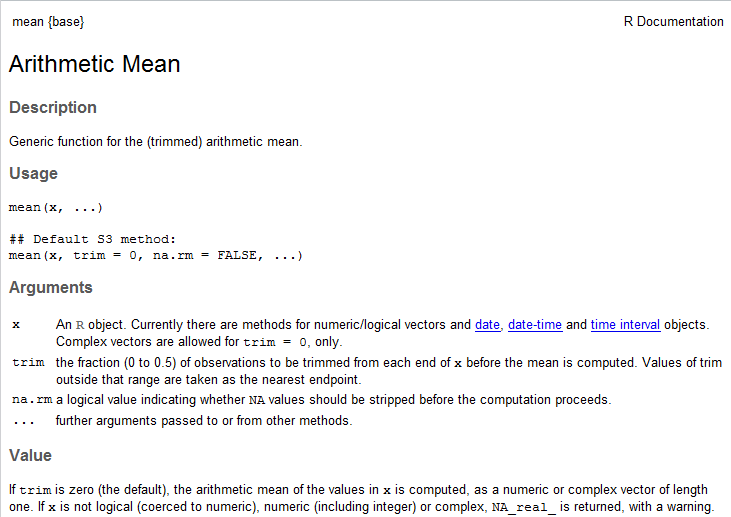
\includegraphics[width = 5in]{mean_help.png}
\end{figure}

Notice the ellipsis (\texttt{...}) after the comma in the \texttt{Usage} section. The ellipsis means that other arguments can be passed to the function. For example, the \texttt{na.rm} argument we covered earlier. However, there are other arguments that we will not cover, and therefore it is best to take on faith that the ellipsis argument will handle whatever it needs to.
\chapter{Descriptive Statistics}
Thus far, all we have covered are functions relating to data and data manipulation. However, R also has many powerful functions for doing statistics. Many of these must be downloaded from packages.
\section{Simple Descriptives}
To find the mean or the median, we simply type \texttt{mean(data)} or \texttt{median(data)}. Many of the other simple functions (\texttt{sum} - compute a sum, \texttt{dim} - return the dimensions of an object) operate in a similar way. 
\section{Other Descriptives and the \texttt{uwIntroStats} package}
For some complex descriptive statistics, as well as some statistical tests and plotting, we will turn to the \texttt{uwIntroStats} package. Developed by Scott S. Emerson, M.D., Ph.D., Andrew J. Spieker, and Brian D. Williamson at the University of Washington, this package seeks to facilitate an easy switch from STATA to R. The functions follow a similar syntax to STATA, and simplify the work of finding some output in R by placing it all in an easy to manage result. However, some of the functions presented come from other R packages (including the base R package).
\section{Summarize vs descrip()}
Quick view of functions:\\
\begin{tabular}{ccc}
STATA & R (base) & R \texttt{uwIntroStats}\\
\hline
\texttt{summarize} & \texttt{summary(), mean(), sd(), var()} & \texttt{descrip()}
\end{tabular}\\
\\
In STATA, a simple summary of the data may be obtained by the \texttt{summarize} command. In R, we have a few different options. In the base package, we can get a good summary of the data by using the \texttt{summary()} function. We can also get simple descriptive statistics using the \texttt{mean(), sd(), var()} and other functions. Or, using the \texttt{uwIntroStats} package, we will use the \texttt{descrip()} function. Details can be found in the documentation for the package. \\
\\Now, for example, we have a data on FEV1 - the volume of air that can be forcibly blown out in one second, after full inspiration - in a clinical trial. This data can be found in the BIOST 511 webpage. Here we illustrate the difference between the STATA and R output:\\

\begin{enumerate}[]
\item \underline{STATA Code and Output}
{\scriptsize
\begin{verbatim}
* Read in data set *
use "https://courses.washington.edu/b511/Data/FEV1ClinTrial.dta"

* Create the table *
summarize

* STATA Output: *
------------------------------------------------------------------------------
Variable |     Obs        Mean     Std. Dev.	Min	   Max
---------+--------------------------------------------------------------------
	      Y1 |     520    1.546192     .6434104   .31    3.75
	      Y0 |	    520    1.521327     .5980118   .33    3.68
	       T |     520    .4961538     .5004667   0      1
------------------------------------------------------------------------------

\end{verbatim}}


\item \underline{R Code and Output}
{\scriptsize
\begin{verbatim}
#- Read in data set -#
clin.trial <- read.table("http://courses.washington.edu/b511/Data/FEV1ClinTrial.dat", sep="")
names(clin.trial) <- c("Y1", "Y0", "T")
attach(clin.trial)

#- Create the table -#
descrip(clin.trial)

#- R Output -# 
      N     Msng  Mean      Std Dev    Min       25%       Mdn       75%       Max     
Y1:     520     0   1.546     0.6434    0.3100    1.060     1.430     1.943     3.750  
Y0:     520     0   1.521     0.5980    0.3300    1.088     1.420     1.910     3.680  
 T:     520     0   0.4962    0.5005    0.0000    0.0000    0.0000    1.000     1.000  
\end{verbatim}}
\end{enumerate}

\chapter{Chi-square Test}
Quick view of functions:\\
\begin{tabular}{ccc}
STATA & R (base) & R \texttt{uwIntroStats}\\
\hline
\texttt{tabulate} & \texttt{chisq.test()} & \texttt{tabulate()}\\
\texttt{cc} & & \\
\texttt{cs} & & \\
\end{tabular}\\
\\
The base R function \texttt{chisq.test} performs the chi-squared test on tables, matrices, and vectors. However, in order to calculate Odds Ratios, Risk Ratios, or other statistics (for example the likelihood ratio, Mantel-Haenszel statistic, and others) you must use other functions developed for different R packages and piece the information together. In our package, the \texttt{tabulate()} function has options for all of these statistics and more. Also, it calculates stratified values if requested. Similar functionality is seen in the STATA command \texttt{tabulate}, or \texttt{cc} and \texttt{cs} (for case control and cohort studies, respectively). We show a few examples to illustrate the performance of the two functions:
\\

\underline{Example 1}:

Data: \texttt{mri}.

Goal: Perform a chi-squared test of stroke vs race.

\begin{enumerate}[]
\item \underline{STATA Code and Output}
{\scriptsize
%import delimited "C:\Users\brian_000\Dropbox\R Project Summer 2014\chisquare\mri.csv"
\begin{verbatim}
* First create csv in Excel using "http://www.emersonstatistics.com/datasets/mri.txt" *
* Read in the data *
import delimited "sample_folder/mri.csv"

* Perform chi-squared test *
tabulate stroke race, chi2


           |                    race
    stroke |         1          2          3          4 |     Total
-----------+--------------------------------------------+----------
         0 |       493         93         39         11 |       636 
         1 |        21          1          2          0 |        24 
         2 |        58         10          6          1 |        75 
-----------+--------------------------------------------+----------
     Total |       572        104         47         12 |       735 

          Pearson chi2(6) =   3.1066   Pr = 0.795

\end{verbatim}}


\item \underline{R Code and Output}
{\scriptsize
\begin{verbatim}
#- If not already done, load the necessary libraries -#
library(survival)
library(Exact)
library(plyr)

#- Read in the data -#
mri <- read.table("http://www.emersonstatistics.com/datasets/mri.txt", header=TRUE, quote="\"")
attach(mri)

#- create the table -#
tabulate(stroke, race)

#- Output -#

Call:
tabulate(stroke, race)
           race.1 race.2 race.3 race.4 race.ALL
stroke.0   493     93     39     11    636     
stroke.1    21      1      2      0     24     
stroke.2    58     10      6      1     75     
stroke.ALL 572    104     47     12    735     
            Point Estimate Test Statistic df 95% CI p-value Warnings
Chi-squared                3.1066         6         0.79536            
\end{verbatim}}

\end{enumerate}

\underline{Example 2}:

Data: \texttt{mri}.

Goal: Perform a chi-squared test of stroke vs race, with row and column percentages displayed.

\begin{enumerate}[]
\item \underline{STATA Code and Output}
{\scriptsize
\begin{verbatim}
* First create csv in Excel using "http://www.emersonstatistics.com/datasets/mri.txt" *
* Read in the data *
import delimited "sample_folder/mri.csv"

* Perform chi-squared test *
tabulate stroke race male, row column chi2

+-------------------+
| Key               |
|-------------------|
|     frequency     |
|  row percentage   |
| column percentage |
+-------------------+

           |                    race
    stroke |         1          2          3          4 |     Total
-----------+--------------------------------------------+----------
         0 |       493         93         39         11 |       636 
           |     77.52      14.62       6.13       1.73 |    100.00 
           |     86.19      89.42      82.98      91.67 |     86.53 
-----------+--------------------------------------------+----------
         1 |        21          1          2          0 |        24 
           |     87.50       4.17       8.33       0.00 |    100.00 
           |      3.67       0.96       4.26       0.00 |      3.27 
-----------+--------------------------------------------+----------
         2 |        58         10          6          1 |        75 
           |     77.33      13.33       8.00       1.33 |    100.00 
           |     10.14       9.62      12.77       8.33 |     10.20 
-----------+--------------------------------------------+----------
     Total |       572        104         47         12 |       735 
           |     77.82      14.15       6.39       1.63 |    100.00 
           |    100.00     100.00     100.00     100.00 |    100.00 

          Pearson chi2(6) =   3.1066   Pr = 0.795

\end{verbatim}}


\item \underline{R Code and Output}
{\scriptsize
\begin{verbatim}
#- Read in the data -#
mri <- read.table("http://www.emersonstatistics.com/datasets/mri.txt", header=TRUE, quote="\"")
attach(mri)

#- create the table -#
tabulate(stroke, race, stat="@count@ @row%@ @col%@")

Call:
tabulate(stroke, race, stat = "@count@ @row%@ @col%@")
           race.1            race.2            race.3            race.4            race.ALL         
stroke.0   493  77.5%  86.2%  93  14.6%  89.4%  39   6.1%  83.0%  11   1.7%  91.7% 636 100.0%  86.5%
stroke.1    21  87.5%   3.7%   1   4.2%   1.0%   2   8.3%   4.3%   0   0.0%   0.0%  24 100.0%   3.3%
stroke.2    58  77.3%  10.1%  10  13.3%   9.6%   6   8.0%  12.8%   1   1.3%   8.3%  75 100.0%  10.2%
stroke.ALL 572  77.8% 100.0% 104  14.1% 100.0%  47   6.4% 100.0%  12   1.6% 100.0% 735 100.0% 100.0%
            Point Estimate Test Statistic df 95% CI p-value Warnings
Chi-squared                3.1066         6         0.79536          

\end{verbatim}}

\end{enumerate}

\underline{Example 3}:

Data: \texttt{mri}.

Goal: Perform a chi-squared test of stroke vs race, with the likelihood ratio rest and exact test displayed.

\begin{enumerate}[]
\item \underline{STATA Code and Output}
{\scriptsize
\begin{verbatim}
* First create csv in Excel using "http://www.emersonstatistics.com/datasets/mri.txt" *
* Read in the data *
import delimited "sample_folder/mri.csv"

* Perform chi-squared test *
tabulate stroke race, chi2 lrchi2 exact

Enumerating sample-space combinations:
stage 4:  enumerations = 1
stage 3:  enumerations = 5
stage 2:  enumerations = 63
stage 1:  enumerations = 0

           |                    race
    stroke |         1          2          3          4 |     Total
-----------+--------------------------------------------+----------
         0 |       493         93         39         11 |       636 
         1 |        21          1          2          0 |        24 
         2 |        58         10          6          1 |        75 
-----------+--------------------------------------------+----------
     Total |       572        104         47         12 |       735 

          Pearson chi2(6) =   3.1066   Pr = 0.795
 likelihood-ratio chi2(6) =   4.1111   Pr = 0.662
           Fisher's exact =                 0.793


\end{verbatim}}


\item \underline{R Code and Output}
{\scriptsize
\begin{verbatim}
#- Read in the data -#
mri <- read.table("http://www.emersonstatistics.com/datasets/mri.txt", header=TRUE, quote="\"")
attach(mri)

#- create the table -#
tabulate(stroke, race, tests=c("lrchisq", "fisher"))

Call:
tabulate(stroke, race, tests = c("lrchisq", "fisher"))
           race.1 race.2 race.3 race.4 race.ALL
stroke.0   493     93     39     11    636     
stroke.1    21      1      2      0     24     
stroke.2    58     10      6      1     75     
stroke.ALL 572    104     47     12    735     
                    Point Estimate Test Statistic df 95% CI p-value Warnings
Chi-squared                        3.1066         6         0.79536         
LR Chi-squared                     4.1111         6         0.66164         
Fisher's Exact Test                                         0.79349 
\end{verbatim}}

\end{enumerate}
\underline{Example 4}:

Data: \texttt{mri}.

Goal: Perform a chi-squared test of diabetes vs male by race, ratios displayed and the Mantel-Haenszel statistic.

\begin{enumerate}[]
\item \underline{STATA Code and Output}
{\scriptsize
\begin{verbatim}
* First create csv in Excel using "http://www.emersonstatistics.com/datasets/mri.txt" *
* Read in the data *
import delimited "sample_folder/mri.csv"

* Perform chi-squared test *
 cc diabetes male, by(race)

            race |       OR       [95% Conf. Interval]   M-H Weight
-----------------+-------------------------------------------------
               1 |     1.9152      1.045652   3.587491     8.741259 (exact)
               2 |   3.284211       .978571   12.68598     1.826923 (exact)
               3 |   2.631579      .1255083   161.3361     .4042553 (exact)
               4 |          .      .2483932          .            0 (exact)
-----------------+-------------------------------------------------
           Crude |   2.233841      1.333028   3.814119              (exact)
    M-H combined |   2.230293      1.358842   3.660624              
-------------------------------------------------------------------
Test of homogeneity (Tarone)   chi2(3) =     1.33  Pr>chi2 = 0.7223

                   Test that combined OR = 1:
                                Mantel-Haenszel chi2(1) =     10.40
                                                Pr>chi2 =    0.0013


\end{verbatim}}


\item \underline{R Code and Output}
{\scriptsize
\begin{verbatim}
#- Read in the data -#
mri <- read.table("http://www.emersonstatistics.com/datasets/mri.txt", header=TRUE, quote="\"")
attach(mri)

#- create the table -#
tabulate(diabetes, male, race, dispRatios=TRUE, tests=c("lrchisq", "mh"))

Call:
tabulate(diabetes, male, race, dispRatios = TRUE, tests = c("lrchisq", 
    "mh"))

 race.1 : 
             male.0 male.1 male.ALL
diabetes.0   266    250    516     
diabetes.1    20     36     56     
diabetes.ALL 286    286    572     
                Point Estimate Test Statistic df 95% CI           p-value  Warnings
Chi-squared                    5.0676         1                   0.024378         
LR Chi-squared                 5.132          1                   0.023489         
Mantel-Haenzsel 2.2303         9.6447         1  [1.36,3.66]      0.001899         
Odds Ratio      1.9152                           [1.0796, 3.3976]                  
Risk Ratio      1.8                              [1.0686, 3.0321]                  

 race.2 : 
             male.0 male.1 male.ALL
diabetes.0    48     38     86     
diabetes.1     5     13     18     
diabetes.ALL  53     51    104     
                Point Estimate Test Statistic df 95% CI           p-value  Warnings
Chi-squared                    4.6816         1                   0.030487         
LR Chi-squared                 4.8099         1                   0.028296         
Mantel-Haenzsel 2.2303         9.6447         1  [1.36,3.66]      0.001899         
Odds Ratio      3.2842                           [1.0761, 10.023]                  
Risk Ratio      2.702                            [1.0376, 7.0362]                  

 race.3 : 
             male.0 male.1 male.ALL
diabetes.0    25     19     44     
diabetes.1     1      2      3     
diabetes.ALL  26     21     47     
                Point Estimate Test Statistic df 95% CI            p-value  Warnings
Chi-squared                    0.62669        1                    0.42857          
LR Chi-squared                 0.62761        1                    0.42823          
Mantel-Haenzsel 2.2303         9.6447         1  [1.36,3.66]       0.001899         
Odds Ratio      2.6316                           [0.22181, 31.221]                  
Risk Ratio      2.4762                           [0.24078, 25.466]                  

 race.4 : 
             male.0 male.1 male.ALL
diabetes.0     4      6     10     
diabetes.1     0      2      2     
diabetes.ALL   4      8     12     
                Point Estimate Test Statistic df 95% CI      p-value  Warnings
Chi-squared                    1.2            1              0.27332          
LR Chi-squared                 1.8161         1              0.17778          
Mantel-Haenzsel 2.2303         9.6447         1  [1.36,3.66] 0.001899         
Odds Ratio      Inf                              [NaN, Inf]                   
Risk Ratio      Inf                              [NaN, Inf]                   

 race.ALL : 
             male.0 male.1 male.ALL
diabetes.0   343    313    656     
diabetes.1    26     53     79     
diabetes.ALL 369    366    735     
                Point Estimate Test Statistic df 95% CI           p-value   Warnings
Chi-squared                    10.588         1                   0.0011384         
LR Chi-squared                 10.777         1                   0.0010279         
Mantel-Haenzsel 2.2303         9.6447         1  [1.36,3.66]      0.001899          
Odds Ratio      2.2338                           [1.3635, 3.6597]                   
Risk Ratio      2.0552                           [1.3151, 3.2118]                   

 Overall:  
                 Test Statistic df p-value   
Chi-squared      22.164         5  0.0004874 
Likelihood Ratio 23.162         5  0.00031429
\end{verbatim}}

\end{enumerate}

\underline{Example 5}:

Data: \texttt{mri}.

Goal: Perform a chi-squared test of diabetes vs male, with Fisher's Exact test and Barnard's Unconditional Exact test displayed.

\begin{enumerate}[]
\item \underline{STATA Code and Output}
{\scriptsize
\begin{verbatim}
* First create csv in Excel using "http://www.emersonstatistics.com/datasets/mri.txt" *
* Read in the data *
import delimited "sample_folder/mri.csv"

* Perform chi-squared test *
tabulate diabetes male, chi2 exact

           |         male
  diabetes |         0          1 |     Total
-----------+----------------------+----------
         0 |       343        313 |       656 
         1 |        26         53 |        79 
-----------+----------------------+----------
     Total |       369        366 |       735 

          Pearson chi2(1) =  10.5877   Pr = 0.001
           Fisher's exact =                 0.001
   1-sided Fisher's exact =                 0.001


\end{verbatim}}

\newpage
\item \underline{R Code and Output}
{\scriptsize
\begin{verbatim}
#- Read in the data -#
mri <- read.table("http://www.emersonstatistics.com/datasets/mri.txt", header=TRUE, quote="\"")
attach(mri)

#- create the table -#
tabulate(diabetes, male, tests=c("fisher", "uWald", "uScore"))

Call:
tabulate(diabetes, male, tests = c("fisher", "uWald", "uScore"))
             male.0 male.1 male.ALL
diabetes.0   343    313    656     
diabetes.1    26     53     79     
diabetes.ALL 369    366    735     
                                 Point Estimate Test Statistic df 95% CI p-value   Warnings
Chi-squared                                     10.588         1         0.0011384         
Fisher's Exact Test                                                      0.0012349         
Unconditional Exact Test (Wald)                 3.4384                   0.13524           
Unconditional Exact Test (Score)                3.2539                   0.0052114    
\end{verbatim}}
\end{enumerate}
\underline{Example 6:}\\
Data: \texttt{mri}
Goal: Print stratified vs overall chi-squared test for stroke vs race by male, with row/column/total percentages calculated.

\underline{R Code and Output}
{\scriptsize
\begin{verbatim}
#- Read in the data -#
mri <- read.table("http://www.emersonstatistics.com/datasets/mri.txt", header=TRUE, quote="\"")
attach(mri)

#- Create the stratified table -#
tabulate(stroke, race, male, stat="@count@ @row%@ @col%@ @tot%@")

Call:
tabulate(stroke, race, male, stat = "@count@ @row%@ @col%@ @tot%@")

 male.0 : 
           race.1                   race.2                   race.3                   race.4                  
stroke.0   255  77.3%  89.2%  34.7%  50  15.2%  94.3%   6.8%  21   6.4%  80.8%   2.9%   4   1.2% 100.0%   0.5%
stroke.1    13  86.7%   4.5%   1.8%   0   0.0%   0.0%   0.0%   2  13.3%   7.7%   0.3%   0   0.0%   0.0%   0.0%
stroke.2    18  75.0%   6.3%   2.4%   3  12.5%   5.7%   0.4%   3  12.5%  11.5%   0.4%   0   0.0%   0.0%   0.0%
stroke.ALL 286  77.5% 100.0%  38.9%  53  14.4% 100.0%   7.2%  26   7.0% 100.0%   3.5%   4   1.1% 100.0%   0.5%
           race.ALL                
stroke.0   330 100.0%  89.4%  44.9%
stroke.1    15 100.0%   4.1%   2.0%
stroke.2    24 100.0%   6.5%   3.3%
stroke.ALL 369 100.0% 100.0%  50.2%
            Point Estimate Test Statistic df 95% CI p-value Warnings
Chi-squared                5.085          6         0.53296         

 male.1 : 
           race.1                   race.2                   race.3                   race.4                  
stroke.0   238  77.8%  83.2%  32.4%  43  14.1%  84.3%   5.9%  18   5.9%  85.7%   2.4%   7   2.3%  87.5%   1.0%
stroke.1     8  88.9%   2.8%   1.1%   1  11.1%   2.0%   0.1%   0   0.0%   0.0%   0.0%   0   0.0%   0.0%   0.0%
stroke.2    40  78.4%  14.0%   5.4%   7  13.7%  13.7%   1.0%   3   5.9%  14.3%   0.4%   1   2.0%  12.5%   0.1%
stroke.ALL 286  78.1% 100.0%  38.9%  51  13.9% 100.0%   6.9%  21   5.7% 100.0%   2.9%   8   2.2% 100.0%   1.1%
           race.ALL                
stroke.0   306 100.0%  83.6%  41.6%
stroke.1     9 100.0%   2.5%   1.2%
stroke.2    51 100.0%  13.9%   6.9%
stroke.ALL 366 100.0% 100.0%  49.8%
            Point Estimate Test Statistic df 95% CI p-value Warnings
Chi-squared                0.94735        6         0.98753         

 male.ALL : 
           race.1                   race.2                   race.3                   race.4                  
stroke.0   493  77.5%  86.2%  67.1%  93  14.6%  89.4%  12.7%  39   6.1%  83.0%   5.3%  11   1.7%  91.7%   1.5%
stroke.1    21  87.5%   3.7%   2.9%   1   4.2%   1.0%   0.1%   2   8.3%   4.3%   0.3%   0   0.0%   0.0%   0.0%
stroke.2    58  77.3%  10.1%   7.9%  10  13.3%   9.6%   1.4%   6   8.0%  12.8%   0.8%   1   1.3%   8.3%   0.1%
stroke.ALL 572  77.8% 100.0%  77.8% 104  14.1% 100.0%  14.1%  47   6.4% 100.0%   6.4%  12   1.6% 100.0%   1.6%
           race.ALL                
stroke.0   636 100.0%  86.5%  86.5%
stroke.1    24 100.0%   3.3%   3.3%
stroke.2    75 100.0%  10.2%  10.2%
stroke.ALL 735 100.0% 100.0% 100.0%
            Point Estimate Test Statistic df 95% CI p-value Warnings
Chi-squared                3.1066         6         0.79536         

 Overall:  
            Test Statistic df p-value
Chi-squared 9.1389         18 0.95644
#- Create the overall table -#
tabulate(stroke, race, male, stratified=FALSE, stat="@count@ @row%@ @col%@ @tot%@")

Call:
tabulate(stroke, race, male, stratified = FALSE, stat = "@count@ @row%@ @col%@ @tot%@")

 male.0 : 
           race.1                     race.2                        race.3                       
stroke.0   255  34.7%  34.7%  34.7%    50  6.8%  6.8%   6.8%         21   2.86%  2.86%   2.86%   
stroke.1    13  1.77%   1.77%   1.77%   0   0%   0%   0%              2  0.272%   0.272%   0.272%
stroke.2    18  2.45%   2.45%   2.45%   3  0.408%   0.408%   0.408%   3  0.408%  0.408%   0.408% 
stroke.ALL 286  38.9% 38.9%  38.9%     53  7.21% 7.21%   7.21%       26   3.54% 3.54%   3.54%    
           race.4                       race.ALL                 
stroke.0     4   0.544% 0.544%   0.544% 330 44.9%  44.9%  44.9%  
stroke.1     0   0%   0%   0%            15 2.04%   2.04%   2.04%
stroke.2     0   0%   0%   0%            24 3.27%   3.27%   3.27%
stroke.ALL   4   0.544% 0.544%   0.544% 369 50.2% 50.2%  50.2%   

 male.1 : 
           race.1                     race.2                        race.3                       
stroke.0   238  32.4%  32.4%  32.4%    43  5.85%  5.85%   5.85%      18   2.45%  2.45%   2.45%   
stroke.1     8  1.09%   1.09%   1.09%   1  0.136%   0.136%   0.136%   0   0%   0%   0%           
stroke.2    40  5.44%  5.44%   5.44%    7  0.952%  0.952%   0.952%    3   0.408%  0.408%   0.408%
stroke.ALL 286  38.9% 38.9%  38.9%     51  6.94% 6.94%   6.94%       21   2.86% 2.86%   2.86%    
           race.4                        race.ALL                 
stroke.0     7   0.952%  0.952%   0.952% 306 41.6%  41.6%  41.6%  
stroke.1     0   0%   0%   0%              9 1.22%   1.22%   1.22%
stroke.2     1   0.136%  0.136%   0.136%  51 6.94%  6.94%   6.94% 
stroke.ALL   8   1.09% 1.09%   1.09%     366 49.8% 49.8%  49.8%   

 male.ALL : 
           race.1                     race.2                         race.3                        
stroke.0   493  67.1%  67.1%  67.1%    93  12.7%  12.7%  12.7%        39   5.31%  5.31%   5.31%    
stroke.1    21  2.86%   2.86%   2.86%   1   0.136%   0.136%   0.136%   2   0.272%   0.272%   0.272%
stroke.2    58  7.89%  7.89%   7.89%   10  1.36%   1.36%   1.36%       6   0.816%  0.816%   0.816% 
stroke.ALL 572  77.8% 77.8%  77.8%    104  14.1% 14.1%  14.1%         47   6.39% 6.39%   6.39%     
           race.4                         race.ALL                 
stroke.0    11   1.5%  1.5%   1.5%        636 86.5%  86.5%  86.5%  
stroke.1     0   0%   0%   0%              24 3.27%   3.27%   3.27%
stroke.2     1   0.136%   0.136%   0.136%  75 10.2%  10.2%  10.2%  
stroke.ALL  12   1.63% 1.63%   1.63%      735 100% 100% 100%       

 Overall:  
            Test Statistic df p-value
Chi-squared 9.1389         18 0.95644
\end{verbatim}}
\chapter{Plots}

\section{Boxplots}
Quick view of functions:\\
\begin{tabular}{ccc}
STATA & R (base) & R \texttt{uwIntroStats}\\
\hline
\texttt{graph box} & \texttt{boxplot()} & \texttt{bplot()}
\end{tabular}\\
\\
Boxplots can be quite controversial as a descriptive plot of the data. Firstly, the population quartiles are most often not the parameters of interest and so the box plot may not provide meaningful insight in answering a scientific question. The definition of an `outlier" as defined by lying 1.5 $\times$ the interquartile range away is indeed arbitrary; we don't have a good sense of what would be a better replacement. With that said, our new R function - \texttt{bplot()} - has many of the the normal capabilities of the default boxplot function (\texttt{boxplot()}), but it is straightforward to: 1) add jittered data to the plot and 2) overlay information about the sample mean and standard deviation. We use the FEV data set as an example.


\begin{enumerate}[]
\item \underline{STATA Code and Output}
{\scriptsize
\begin{verbatim}
* Read in data set *
use "https://courses.washington.edu/b511/Data/FEV1ClinTrial.dta"

* Box Plot *
graph box fev, by(smoke) ytitle(“FEV”)

* STATA Output: *
\end{verbatim}}
\begin{figure}[h!]
\centering
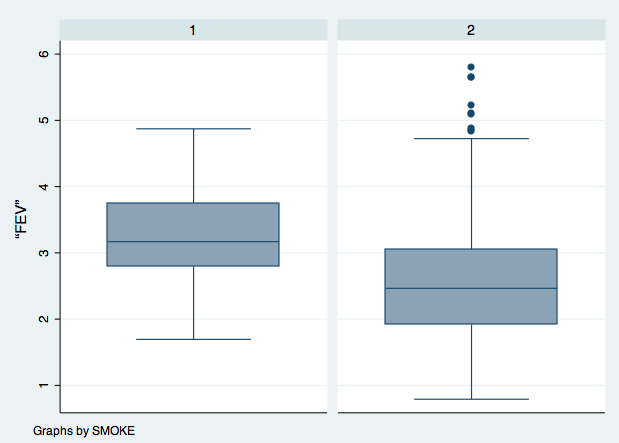
\includegraphics[width = 10cm]{FEVbplotSt.png}
\end{figure}
\newpage
\item \underline{R Code and Output}
{\scriptsize
\begin{verbatim}
#- Read in data set -#
fev <- read.table("http://courses.washington.edu/b511/Data/FEV1ClinTrial.dat", sep="")
attach(fev)

#- Box Plot -#
bplot(y = FEV, x = SMOKE, xlab = "Smoking Group", ylab = "FEV")

#- R Output -# 
\end{verbatim}}
\begin{figure}[h!]
\centering
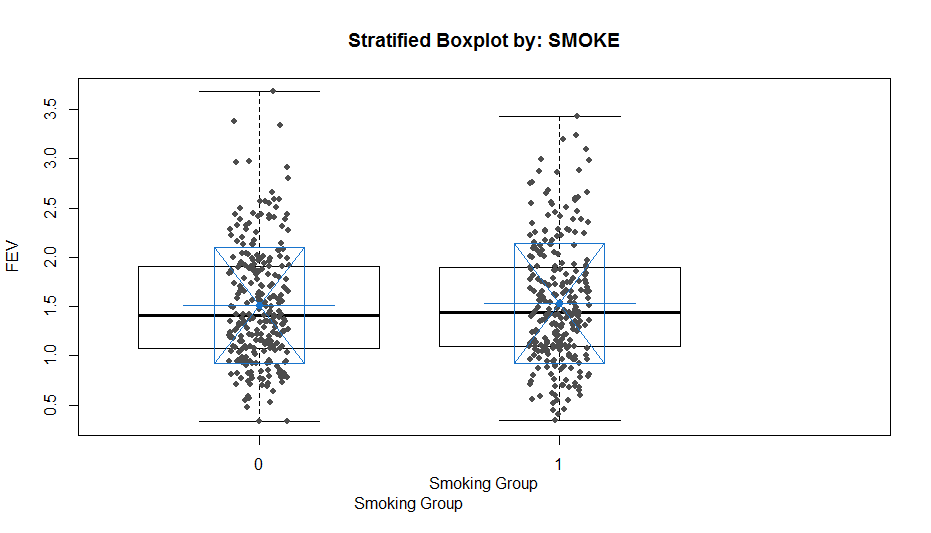
\includegraphics[width = 10cm]{FEVbplotR.png}
\end{figure}
\end{enumerate}
\newpage
\section{Histograms}
Quick view of functions:\\
\begin{tabular}{cc}
STATA & R (base) \\
\hline
\texttt{histogram} & \texttt{hist()}
\end{tabular}\\
\\
The syntax for histograms is very similar between STATA and the base R package. However, in R, we must label the axes. Thus we use the \texttt{ylab} and \texttt{xlab} arguments to apply a y and x-axis label to the plot. The \texttt{breaks} command allows us to enter the number of bins we want displayed on the histogram.
\begin{enumerate}[]
\item \underline{STATA Code and Output}
{\scriptsize
\begin{verbatim}
* Read in data set *
use "https://courses.washington.edu/b511/Data/FEV1ClinTrial.dta"

* Create a histogram *
histogram Y1

* STATA Output: *
\end{verbatim}}
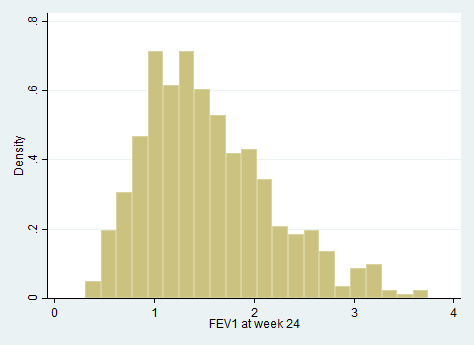
\includegraphics[height=2in, width=2in]{fev1hist.png}
{\scriptsize
\begin{verbatim}
* Save the graph *
graph export "test directory\example1.png"
\end{verbatim}}
\item \underline{R Code and Output}
{\scriptsize
\begin{verbatim}
#- Read in data set -#
clin.trial <- read.table("http://courses.washington.edu/b511/Data/FEV1ClinTrial.dat", sep="")
names(clin.trial) <- c("Y1", "Y0", "T")
attach(clin.trial)

#- Create a histogram -#
hist(Y1, ylab="Frequency", xlab="FEV1 at 24 Weeks", main="Histogram of FEV1 at 24 Weeks")

#- R Output -# 
\end{verbatim}}
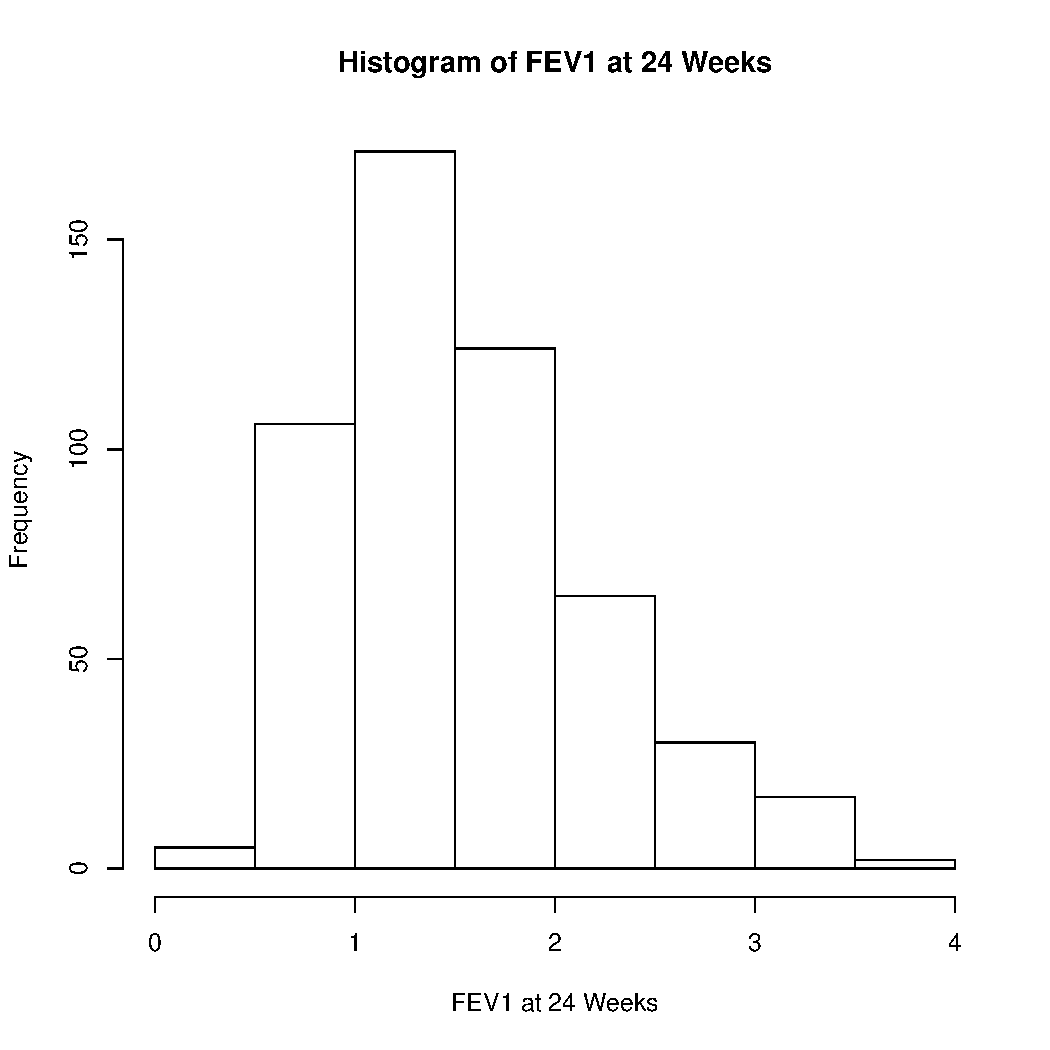
\includegraphics[height=2in, width=2in]{fev1hist_R.pdf}
{\scriptsize
\begin{verbatim}
#- Save the graph -#
pdf(file="testdirectory/example1.pdf")
> hist(Y1, ylab="Frequency", xlab="FEV1 at 24 Weeks", main="Histogram of FEV1 at 24 Weeks")
> dev.off()

#- Version with 22 bins -#
hist(Y1, ylab="Frequency", xlab="FEV1 at 24 Weeks", main="Histogram of FEV1 at 24 Weeks", breaks=22)
\end{verbatim}}
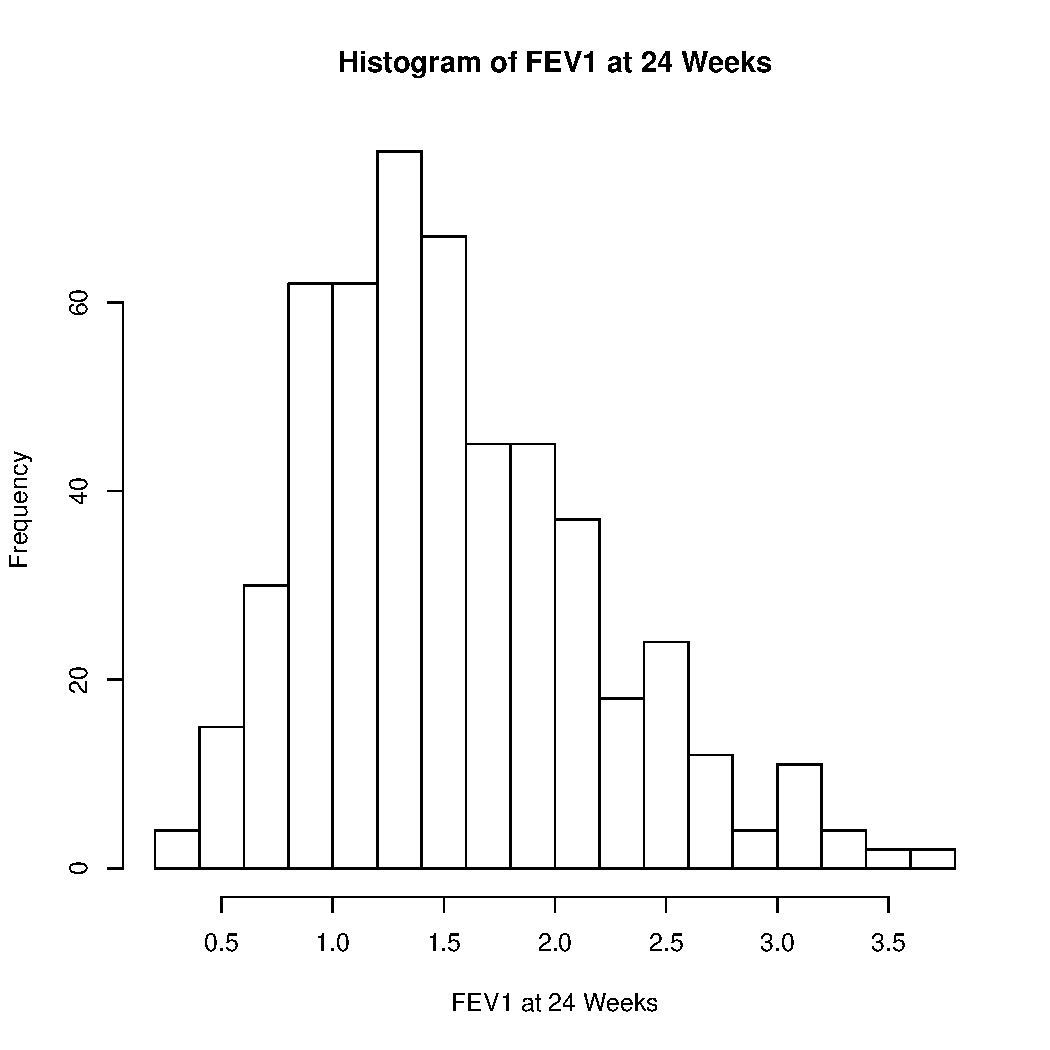
\includegraphics[height=2in, width=2in]{fev1hist_R2.pdf}
{\scriptsize
\begin{verbatim}
#- Save the graph -#
pdf(file="testdirectory/example1.pdf")
hist(Y1, ylab="Frequency", xlab="FEV1 at 24 Weeks", main="Histogram of FEV1 at 24 Weeks", breaks=22)
dev.off()
\end{verbatim}}
\end{enumerate}
\section{Scatterplots}
Quick view of functions:\\
\begin{tabular}{ccc}
STATA & R (base) & R \texttt{uwIntroStats}\\
\hline
\texttt{scatter} & \texttt{plot()} & \texttt{scatter()}
\end{tabular}\\
\\
The base R version of the scatterplot takes an \texttt{x} and a \texttt{y} variable (which must be of the same length) and plots the points as specified by these coordinates. If you wish to have least squares lines or other additions to the plot, you must use the \texttt{abline()} function. The STATA version of scatterplot and the R version (in our package) of scatterplot are very similar. The syntax in each is y-variable followed by x-variable, followed by any arguments. However, in our version there are some extra arguments that need to be added to the function call in order to get exactly what we want.
\begin{enumerate}[]
\item \underline{STATA Code and Output}
{\scriptsize
\begin{verbatim}
* Read in data set *
use "https://courses.washington.edu/b511/Data/FEV1ClinTrial.dta"

* Create a scatterplot with lowess curves and least squares fitted regression lines *
scatter Y1 Y0 || lfit Y1 Y0 || lowess Y1 Y0

* STATA Output: *
\end{verbatim}}
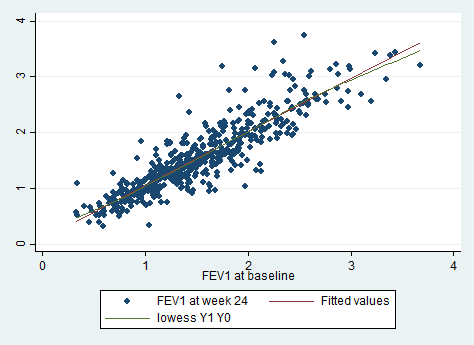
\includegraphics[height=2in, width=2in]{fev1clintrial_lowess_scatter_example1_stata.png}
{\scriptsize
\begin{verbatim}
* Save the graph *
graph export "test directory\example1.png"
\end{verbatim}}
\item \underline{R Code and Output}
{\scriptsize
\begin{verbatim}
#- Read in data set -#
clin.trial <- read.table("http://courses.washington.edu/b511/Data/FEV1ClinTrial.dat", sep="")
names(clin.trial) <- c("Y1", "Y0", "T")
attach(clin.trial)

#- Create a scatterplot with lowess curves and least squares fitted regression lines -#
scatter(Y1, Y0, ylab="FEV1 At 24 Weeks", xlab="FEV1 at Baseline")

#- R Output -# 
\end{verbatim}}
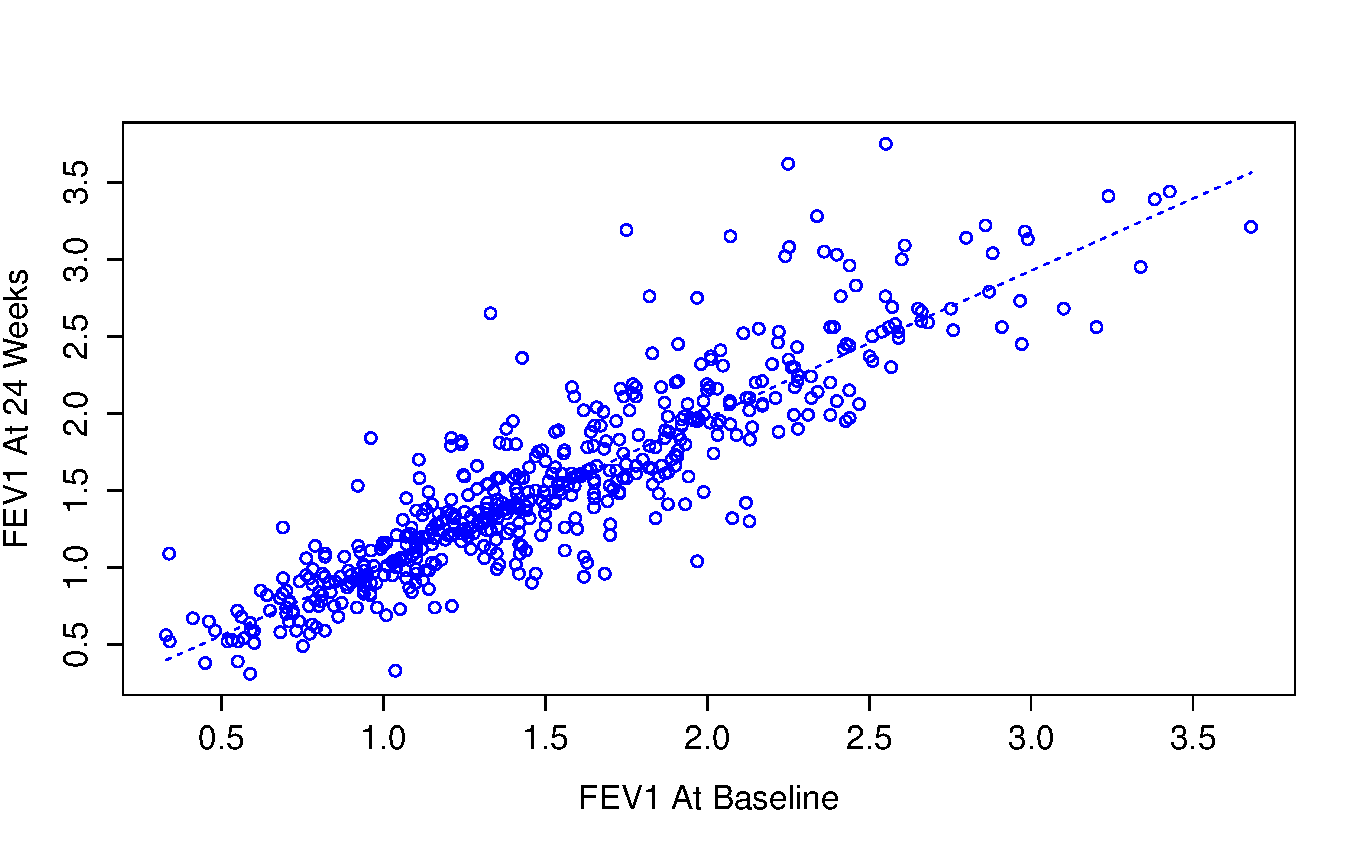
\includegraphics[height=2in, width=2in]{fev1clintrial_lowess_scatter_example1_R.pdf}
{\scriptsize
\begin{verbatim}
#- Save the graph -#
pdf(file="test directory\example1.pdf")
scatter(Y1, Y0, ylab="FEV1 At 24 Weeks", xlab="FEV1 at Baseline")
dev.off()
\end{verbatim}}
\end{enumerate}
\chapter{Correlations}
Quick view of functions:\\
\begin{tabular}{ccc}
STATA & R (base) & R \texttt{uwIntroStats}\\
\hline
\texttt{correlate} & \texttt{cor()} - correlation & \texttt{correlate()}\\
 & \texttt{cov()} - covariance & 
\end{tabular}\\
\\
In STATA, the command to compute a correlation matrix is \texttt{correlate}. In our package, the function called is \texttt{correlate()} and it follows much of the same syntax. The basic function takes in an arbitrary number of variables and returns the correlation matrix, calculating Pearson's correlation coefficient. Note that STATA will not display one of the diagonal elements since the two values are the same, while R does display it. 
\begin{enumerate}[]
\item \underline{STATA Code and Output}
{\scriptsize
\begin{verbatim}
* Read in data set *
use "https://courses.washington.edu/b511/Data/FEV1ClinTrial.dta"

* Calculate the correlation matrix between Y1 and Y0 *
correlate Y1 Y0

* STATA Output: *
(obs=520)

             |       Y1       Y0
-------------+------------------
          Y1 |   1.0000
          Y0 |   0.8932   1.0000

\end{verbatim}}
\item \underline{R Code and Output}
{\scriptsize
\begin{verbatim}
#- Read in data set -#
clin.trial <- read.table("http://courses.washington.edu/b511/Data/FEV1ClinTrial.dat", sep="")
names(clin.trial) <- c("Y1", "Y0", "T")
attach(clin.trial)

#- Calculate the correlation matrix -#
correlate(Y1, Y0)

#- R Output -# 
Tabled correlation statistics by strata
Call:
      correlate(Y1, Y0) 
     Method:  Pearson 
     Data  :  Pairwise Complete 
            - NaN denotes strata with no observations
            - NA arises from missing data

##### ALL DATA
   ##  Estimated Correlation Coefficients 
     Y1:     Y0:    
Y1:   1.0000  0.8932
Y0:   0.8932  1.0000
\end{verbatim}}
\end{enumerate}
\section{Pairwise Correlations}
The command to compute pairwise correlations in STATA is \texttt{pwcorr}. In R, using our package, you simply add the \texttt{use="pairwise.complete.obs"} argument in the \texttt{correlate()} function. If you are using the base R functions, the arguments are the same. If \texttt{"pairwise.complete.obs"} is entered, then the pairwise correlations are computed using all cases that are not missing data. In the examples presented below, there will be no difference between using pairwise correlation and standard correlation coefficients.
\begin{enumerate}[]
\item \underline{STATA Code and Output}
{\scriptsize
\begin{verbatim}
* Read in data set *
use "https://courses.washington.edu/b511/Data/FEV1ClinTrial.dta"

* Calculate the pairwise correlation matrix between Y1 and Y0 *
 pwcorr Y1 Y0

* STATA Output: *

             |       Y1       Y0
-------------+------------------
          Y1 |   1.0000 
          Y0 |   0.8932   1.0000 

\end{verbatim}}
\item \underline{R Code and Output}
{\scriptsize
\begin{verbatim}
#- Read in data set -#
clin.trial <- read.table("http://courses.washington.edu/b511/Data/FEV1ClinTrial.dat", sep="")
names(clin.trial) <- c("Y1", "Y0", "T")
attach(clin.trial)

#- Calculate the pairwise correlation matrix -#
correlate(Y1, Y0, use="pairwise.complete.obs")

#- R Output -# 
Tabled correlation statistics by strata
Call:
      correlate(Y1, Y0, use = "pairwise.complete.obs") 
     Method:  Pearson 
     Data  :  Pairwise Complete 
            - NaN denotes strata with no observations
            - NA arises from missing data

##### ALL DATA
   ##  Estimated Correlation Coefficients 
     Y1:     Y0:    
Y1:   1.0000  0.8932
Y0:   0.8932  1.0000
\end{verbatim}}
\end{enumerate}
\chapter{Cumulative Distribution Functions}
Say we calculate a test statistic (z-score, t-statistic, chi-squared statistic) and want to find the p-value. Recall that for a p-value we want to find the probability of values at least as extreme as our value. Thus in STATA, if we have a z-score of 1, the correct command is \texttt{display 1-normprob(1)}. In R, the function is \texttt{1-pnorm(1)}. Similar functions - \texttt{p} followed by the name of the distribution - can be found for many of the probability distributions.
\begin{enumerate}[]
\item \underline{STATA Code and Output}
{\scriptsize
\begin{verbatim}
* Calculate the p-value for a z-score of 1 *
display normprob(1)

* STATA Output: *
.15865525
\end{verbatim}}
\item \underline{R Code and Output}
{\scriptsize
\begin{verbatim}
#- Calculate the p-value -#
1-pnorm(1)

#- R Output -# 
[1] 0.1586553
\end{verbatim}}
\end{enumerate}


\chapter{One-Sample Inference}

\section{The one-sample t-test}
Quick view of functions:\\
\begin{tabular}{ccc}
STATA & R (base) & R \texttt{uwIntroStats}\\
\hline
\texttt{ttest} & \texttt{t.test()} & \texttt{ttest()}\\
\texttt{ttesti} &  & \texttt{ttesti()}
\end{tabular}\\
\\

R has a default function called \texttt{t.test} which performs a one-sample t-test. The information printed by this default function is not presented in a way that is as clear as that provided by STATA. As part of our package, we provide a t-test function called \texttt{ttest}, which prints a summary comparable in style to that provided by STATA. We also have added on the capability to do tests on geometric means, and to stratify the analysis on given variables.\\

STATA also has an option to run an ``immediate'' t-test, given counts and the sample means and standard deviations. We have implemented a similar function in R. The command in STATA is \texttt{ttesti}, and our function is called \texttt{ttesti()}.

As an example, we consider the WCGS data below and test the hypothesis that that the mean weight in the sampled population is equal to 169 lbs against the (two-sided) alternative that the mean weight is not equal to 169 lbs. STATA provides inference for each one-sided hypothesis. In R, the default is a two-sided test if none is specified by the user, but one may specify the test type with the argument \texttt{test.type} by providing either ``less" or ``greater" instead of ``two.sided".

\begin{enumerate}[]
\item \underline{STATA Code and Output}
{\scriptsize
\begin{verbatim}
* Read in the data *
use ".../wcgs.dta"
* Edit the data if necessary *

* Perform a one-sample t-test on weight *
ttest weight == 169

* STATA Output: *

One-sample t test
------------------------------------------------------------------------------
Variable |     Obs        Mean    Std. Err.   Std. Dev.   [95% Conf. Interval]
---------+--------------------------------------------------------------------
  weight |    3154    169.9537    .3756335    21.09576    169.2172    170.6902
------------------------------------------------------------------------------
    mean = mean(weight)                                           t =   2.5389
Ho: mean = 169                                   degrees of freedom =     3153

   Ha: mean < 169               Ha: mean != 169               Ha: mean > 169
 Pr(T < t) = 0.9944         Pr(|T| > |t|) = 0.0112          Pr(T > t) = 0.0056


\end{verbatim}}
\item \underline{R Code and Output}
{\scriptsize
\begin{verbatim}
#- Read in the data -#
setwd("~/Desktop")
WCGS <- read.csv("WCGS.csv")

#- Attaching the data -#
attach(WCGS)

#- Perform a one-sample t-test on weight -#
ttest(weight, null.hypoth = 169)

#- R Output -#

Call:
ttest(var1 = weight, null.hypoth = 169)

One-sample t-test :
 
Summary:
 Variable  Obs Missing Mean Std. Err. Std. Dev.     95% CI
   weight 3154       0  170     0.376      21.1 [169, 171]

 Ho:  mean = 169 ; 
 Ha:  mean != 169 
 t = 2.539 , df = 3153 
 Pr(|T| > t) =  0.0111667 

\end{verbatim}}
\end{enumerate}

\chapter{Two-Sample Inference}

\section{The two-sample t-test}
Just as the \texttt{ttest} command in STATA is equipped to handle both one- and two-sample inference, the \texttt{ttest} (and \texttt{t.test}) function in R can be used for the two-sample t-test. By default, this function performs a t-test which allows for the possibility that the groups have unequal variances (provided it is not a matched-pairs test, for which that is not an option). This is different from the default in STATA which is to presume that the two groups have equal variances. We consider an example from the WCGS data set.\\

\begin{enumerate}[]
\item \underline{STATA Code and Output}
{\scriptsize
\begin{verbatim}
* Read in the data *
use ".../shoulder_wide.dta"

* Perform a two-sample t-test on SBP by dibpat *
ttest sbp, by(dibpat) unequal

* STATA Output: *

Two-sample t test with unequal variances
------------------------------------------------------------------------------
   Group |     Obs        Mean    Std. Err.   Std. Dev.   [95% Conf. Interval]
---------+--------------------------------------------------------------------
   B3,B4 |    1565    127.4658    .3646562    14.42583    126.7505    128.1811
   A1,A2 |    1589    129.7823    .3935908    15.68942    129.0102    130.5543
---------+--------------------------------------------------------------------
combined |    3154    128.6328     .269188    15.11773     128.105    129.1606
---------+--------------------------------------------------------------------
    diff |           -2.316438    .5365518               -3.368466    -1.26441
------------------------------------------------------------------------------
    diff = mean(B3,B4) - mean(A1,A2)                              t =  -4.3173
Ho: diff = 0                     Satterthwaite's degrees of freedom =  3137.24

    Ha: diff < 0                 Ha: diff != 0                 Ha: diff > 0
 Pr(T < t) = 0.0000         Pr(|T| > |t|) = 0.0000          Pr(T > t) = 1.0000



\end{verbatim}}
\item \underline{R Code and Output}
{\scriptsize
\begin{verbatim}
#- Read in the data -#
setwd("~/Desktop")
WCGS <- read.csv("WCGS.csv")

#- Attaching the data -#
attach(WCGS)

#- Perform a two- sample t-test on pain (matched) -#
ttest(sbp, by = dibpat)

#- R Output -#

Call:
ttest(var1 = sbp, by = dibpat)

Two-sample t-test allowing for unequal variances :
 
Summary:
            Group  Obs Missing   Mean Std. Err. Std. Dev.           95% CI
   dibpat = A1,A2 1589       0 129.78     0.394      15.7 [129.01, 130.55]
   dibpat = B3,B4 1565       0 127.47     0.365      14.4 [126.75, 128.18]
       Difference 3154       0   2.32     0.537      <NA>     [1.26, 3.37]

 Ho: difference in  means = 0 ; 
 Ha: difference in  means != 0 
 t = 4.317 , df = 3137 
 Pr(|T| > t) =  1.62861e-05 

\end{verbatim}}
\end{enumerate}

\chapter{Linear Regression}
Quick view of functions:\\
\begin{tabular}{ccc}
STATA & R (base) & R \texttt{uwIntroStats}\\
\hline
\texttt{regress} & \texttt{lm()} & \texttt{regress()}\\
\end{tabular}\\
\\
In both STATA and our regression function in R, the syntax is dependent variable (y) followed by independent variable (x). The correct STATA command is \texttt{regress}, while the function in R is \texttt{regress()} (or \texttt{reg()}). However, we must specify some of the arguments to \texttt{regress()} before we use it. First is the \texttt{fnctl} argument. This allows the user to specify the desired summary measure of the distribution - acceptable choices are \texttt{"mean"}, \texttt{"geometric mean"}, \texttt{"odds"}, \texttt{"rate"}, and \texttt{"hazard"}. Next, the dependent variable is entered. Last, the independent variables are entered (in vector, matrix, or list of variables). If the \texttt{reg()} function is called, then no functional needs to be entered. It will perform regression on the mean by default.
\newline Also, the \texttt{regress()} function relies on the \texttt{sandwich} package to compute robust standard errors (requested by default), so install and load it if you do not already have it loaded.

\begin{enumerate}[]
\item \underline{STATA Code and Output}
{\scriptsize
\begin{verbatim}
* Read in the data *
import delimited "http://www.emersonstatistics.com/datasets/mri.txt", delimiters("whitespace", collapse)
* Edit the data if necessary *

* Perform the regression *
regress stroke race male

* STATA Output: *

      Source |       SS       df       MS              Number of obs =     735
-------------+------------------------------           F(  2,   732) =    4.23
       Model |  3.22884311     2  1.61442156           Prob > F      =  0.0150
    Residual |   279.57932   732  .381938962           R-squared     =  0.0114
-------------+------------------------------           Adj R-squared =  0.0087
       Total |  282.808163   734  .385297225           Root MSE      =  .61801

------------------------------------------------------------------------------
      stroke |      Coef.   Std. Err.      t    P>|t|     [95% Conf. Interval]
-------------+----------------------------------------------------------------
        race |  -.0014108   .0342548    -0.04   0.967    -.0686601    .0658385
        male |   .1325506   .0455919     2.91   0.004     .0430442    .2220571
       _cons |   .1725898   .0554123     3.11   0.002     .0638039    .2813758
------------------------------------------------------------------------------

\end{verbatim}}
\item \underline{R Code and Output}
{\scriptsize
\begin{verbatim}
#- Read in the data -#
mri <- read.table("http://www.emersonstatistics.com/datasets/mri.txt", 
                  header=TRUE, quote="\"")
#- Attaching the data -#
attach(mri)

#- Regressing stroke vs race and male (and calculating based on the mean) -#
regress("mean", stroke~race+male)


#- R Output -#
Call:
regress(fnctl = "mean", formula = stroke ~ race + male)

Residuals:
    Min      1Q  Median      3Q     Max 
-0.3037 -0.3037 -0.1712 -0.1712  1.8316 

Coefficients:
                 Estimate   Naive SE  Robust SE    95%L      95%H         F stat    df Pr(>F)   
[1] Intercept      0.1726    0.05541   0.05248      0.06956    0.2756         10.81 1    0.0011 
[2] race         -1.411e-03  0.03425   0.03484     -0.06981   0.06699          0.00 1    0.9677 
[3] male           0.1326    0.04559   0.04565      0.04293    0.2222          8.43 1    0.0038 

Residual standard error: 0.618 on 732 degrees of freedom
Multiple R-squared:  0.01142,	Adjusted R-squared:  0.008716 
F-statistic: 4.217 on 2 and 732 DF,  p-value: 0.0151
\end{verbatim}}
\end{enumerate}
\chapter{Regression on Functionals other than the Mean}
Quick view of functions:\\
\begin{tabular}{ccc}
STATA & R (base) & R \texttt{uwIntroStats}\\
\hline
\texttt{regress} & \texttt{lm()} & \texttt{regress()}\\
\end{tabular}\\
\\
The functionals listed above are listed above regress on the functional listed in the name of the function. They produce similar output to those in the previous chapter. 

\chapter{Graphical User Interfaces}
Often, it is more convenient to use a graphical user interface (GUI) rather than use R from the command line. STATA comes pre-loaded with a GUI, and R does too. Typing functions in the GUI is exactly the same as typing in the command line, but the GUI presents everything in a way that is easier to understand and follow. GUIs also provide buttons and tabs that do some useful tasks for the user.
\section{The Basic R GUI}
When you install R, it will usually ask to install a shortcut for R on your desktop. If you use the R application this way (or from the Start menu for Windows users or from the Applications folder for Macintosh users) the basic R GUI will open up. It looks something like this:
\newline
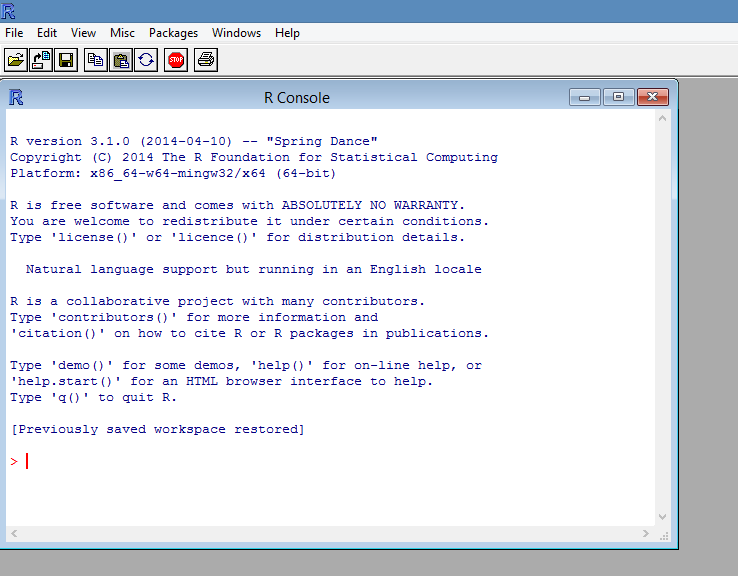
\includegraphics[width=2in, height=2in]{rgui_basic.png}
\newline 
The tabs at the top all have fairly self explanatory functions, from creating and saving scripts to loading packages. The scripts and any plots that are generated appear in the grey space in the GUI window. The main console opens up and is titled ``R Console''. 
\section{RStudio}
There are many other GUIs for R, but a very intuitive one is called RStudio. It can be downloded from www.rstudio.com for free. Before you download RStudio, you must have a version of R downloaded already. You must tell RStudio when you are initially setting it up which version of R to look to. RStudio has all of the same functionality as the basic R GUI, but adds nice features such as the ``Import Dataset'' button which, given the path to a file on your computer or on the internet, downloads and formats the data for you.
\chapter{Examples from Lectures}
\section{BIOST 511 (Taught by David Yanez, Autumn 2013)}
\subsection{Variance and Standard Deviation - Slide 51}
Data: Two samples - 
\newline \texttt{20, 23, 34, 26, 30, 22, 40, 38, 37}
\newline \texttt{30, 29, 30, 31, 32, 30, 28, 30, 30}
\newline Goal: Obtain measures of spread (variance and standard deviation) and a stem and leaf plot.
\begin{enumerate}[]
\item \underline{STATA Code and Output}
{\scriptsize
\begin{verbatim}
* Type in the data *
generate var1 = 20 in 1
replace var1 = 23 in 2
replace var1 = 34 in 3
replace var1 = 26 in 4
replace var1 = 30 in 5
replace var1 = 22 in 6
replace var1 = 40 in 7
replace var1 = 38 in 8
replace var1 = 37 in 9
generate var2 = 30 in 1
replace var2 = 29 in 2
replace var2 = 30 in 3
replace var2 = 31 in 4
replace var2 = 32 in 5
replace var2 = 30 in 6
replace var2 = 28 in 7
replace var2 = 30 in 8
replace var2 = 30 in 9
rename var1 sample1
rename var2 sample2

* Get the variance and standard deviation *
summarize sample1, detail
summarize sample2, detail

* STATA Output: *

                           sample1
-------------------------------------------------------------
      Percentiles      Smallest
 1%           20             20
 5%           20             22
10%           20             23       Obs                   9
25%           23             26       Sum of Wgt.           9

50%           30                      Mean                 30
                        Largest       Std. Dev.      7.566373
75%           37             34
90%           40             37       Variance          57.25
95%           40             38       Skewness              0
99%           40             40       Kurtosis       1.437587



                           sample2
-------------------------------------------------------------
      Percentiles      Smallest
 1%           28             28
 5%           28             29
10%           28             30       Obs                   9
25%           30             30       Sum of Wgt.           9

50%           30                      Mean                 30
                        Largest       Std. Dev.      1.118034
75%           30             30
90%           32             30       Variance           1.25
95%           32             31       Skewness              0
99%           32             32       Kurtosis           3.06

\end{verbatim}}
\item \underline{R Code and Output}
{\scriptsize
\begin{verbatim}
#- Type in the data -#
sample1 <- c(20, 23, 34, 26, 30, 22, 40, 38, 37)
sample2 <- c(30, 29, 30, 31, 32, 30, 28, 30, 30)

#- Get variance and standard deviation -#
descrip(sample1)
#- sd is 4th column of matrix, variance is sd^2 -#
(descrip(sample1)[,4])^2
descrip(sample2)
(descrip(sample2)[,4])^2
#- R Output -#
           N     Msng  Mean      Std Dev    Min       25%       Mdn       75%       Max     
sample1:       9     0   30.00     7.566     20.00   23.000000   30.00     37.00     40.00  

[1] 57.25

           N     Msng  Mean      Std Dev    Min       25%       Mdn       75%       Max     
sample2:       9     0   30.00     1.118     28.00   30.000000   30.00     30.00     32.00  

[1] 1.25
\end{verbatim}}
\end{enumerate}
\subsection{Calculating Quantiles and Percentiles - Slide 53}
Data: ages, \texttt{20, 23, 34, 26, 30, 22, 40, 38, 37}
\newline Goal: Calculate 25th and 75th percentile
\begin{enumerate}[]
\item \underline{STATA Code and Output}
{\scriptsize
\begin{verbatim}
* Type in the data *
generate var1 = 20 in 1
replace var1 = 23 in 2
replace var1 = 34 in 3
replace var1 = 26 in 4
replace var1 = 30 in 5
replace var1 = 22 in 6
replace var1 = 40 in 7
replace var1 = 38 in 8
replace var1 = 37 in 9
rename var1 age

* Get centiles *
centile age, centile(25 50 75)
* STATA Output: *
                                                       -- Binom. Interp. --
    Variable |     Obs  Percentile      Centile        [95% Conf. Interval]
-------------+-------------------------------------------------------------
         age |       9         25          22.5              20    32.45832*
             |                 50            30        22.07778    37.92222
             |                 75          37.5        27.54168          40*

\end{verbatim}}
\item \underline{R Code and Output}
{\scriptsize
\begin{verbatim}
#- Read in the data -#
age <- c(20, 23, 34, 26, 30, 22, 40, 38, 37)

#- Get centiles (25, 50, 75) -#
descrip(age)

#- R Output -#
       N     Msng  Mean      Std Dev    Min       25%       Mdn       75%       Max     
age:       9     0   30.00     7.566     20.00   23.000000   30.00     37.00     40.00  
\end{verbatim}}
\end{enumerate}
\subsection{2x2 Table - Slide 110}
Data: Pauling (1971) Vitamin C data
\newline Goal: Determine if there is an association between treatment and disease.
\begin{enumerate}[]
\item \underline{STATA Code and Output}
{\scriptsize
\begin{verbatim}
* Run case-control chi-squared test *
cci 17 122 31 109
* STATA Output: *

                                                         Proportion
                 |   Exposed   Unexposed  |      Total     Exposed
-----------------+------------------------+------------------------
           Cases |        17         122  |        139       0.1223
        Controls |        31         109  |        140       0.2214
-----------------+------------------------+------------------------
           Total |        48         231  |        279       0.1720
                 |                        |
                 |      Point estimate    |    [95% Conf. Interval]
                 |------------------------+------------------------
      Odds ratio |         .4899524       |    .2407003    .9744098 (exact)
 Prev. frac. ex. |         .5100476       |    .0255902    .7592997 (exact)
 Prev. frac. pop |         .1129391       |
                 +-------------------------------------------------
                               chi2(1) =     4.81  Pr>chi2 = 0.0283

\end{verbatim}}
\item \underline{R Code and Output}
{\scriptsize
\begin{verbatim}
#- Set data -#
vitaminC <- c(rep(1, 17), rep(0, 122))
placebo <- c(rep(1, 31), rep(0, 109))
#- Run case-control chi-squared -#
tabulate(vitaminC, placebo, dispRatios=TRUE)
#- R Output -#

\end{verbatim}}
\end{enumerate}
\subsection{Next Example}
Data:
\newline Goal:
\begin{enumerate}[]
\item \underline{STATA Code and Output}
{\scriptsize
\begin{verbatim}
* Type in the data *

* STATA Output: *

\end{verbatim}}
\item \underline{R Code and Output}
{\scriptsize
\begin{verbatim}
#- Read in the data -#

#- R Output -#

\end{verbatim}}
\end{enumerate}

\section{BIOST 514/517 (Taught by Katie Kerr, Autumn 2013)}
\subsubsection{Basic Summary Statistics - Lecture 04}
$$\begin{tabular}{rll}
\multicolumn{3}{l}{}\\ \hline
\textbf{STATA Command} & \textbf{Syntax} & \textbf{Desription}\\ \hline
\texttt{describe} & describe \textit{varlist} & type of variable; value labels \\
\texttt{inspect} & inspect \textit{varlist} & crude hist; msg; integer; counts sign \\
\texttt{summarize} & summarize \textit{varlist}, format & non msg, mean, sd, min, max \\
\texttt{summarize} & summarize \textit{varlist}, detail format & plus quantiles, skewness, kurtosis \\
\texttt{means} & means \textit{varlist} & artith., geom., harm. means, nonmsg, CI \\
\texttt{centile} & centile \textit{varlist}, cen(x, y) & table of requested quant., CI \\
\texttt{tabstat} & tabstat \textit{varlist}, stat(n mean sd & table of relevant stats for var \\
~ & min p25 med p75 max) & \\
\texttt{tabulate} & tabulate \textit{var} & frequency for variables \\
\hline
\end{tabular}$$\\
$$\begin{tabular}{rll}
\multicolumn{3}{l}{}\\ \hline
\textbf{R Command} & \textbf{Syntax} & \textbf{Desription}\\ \hline
\texttt{descrip} & descrip \textit{varlist} & descriptive statistics of the variables entered \\
 & & if requested, displays count of msng, mean, geom mean, sd, min, max, \\
  & & quantiles, CI, frequency\\ 
\hline
\end{tabular}$$\\

\textit{Procedures:}
\begin{enumerate}[1.]
\item Dichotomizing data - STATA
	\begin{itemize}
		\item \texttt{generate} x = 0
		\item \texttt{replace} x = 1 if y $\geq$5
	\end{itemize}
\item Dichotomizing data - R
	\begin{itemize}
		\item \texttt{x <- ifelse(y $\geq$ 5, 1, 0)}
	\end{itemize}
\item Computing the mode (discrete) - STATA
	\begin{itemize}
		\item \texttt{table} \textit{var}
		\item Examine output for highest frequency
	\end{itemize}
\item Computing the mode (discrete) - R
	\begin{itemize}
		\item \texttt{table}(\textit{var})
		\item Examine output for highest frequency
	\end{itemize}
\item Computing the mode (continuous) - STATA
	\begin{itemize}
		\item \texttt{kdensity} \textit{var}, g(x d)
	\end{itemize}
	\item Computing the mode (continuous) - R
	\begin{itemize}
		\item \texttt{x <- density(}\textit{var}\texttt{)}\\
				\texttt{plot(x)}
		\item Examine plot for highest frequency
	\end{itemize}
\end{enumerate}

\section{Autumn 2014}
More examples from lecture (BIOST 511 taught by Lurdes Inoue and BIOST 514/517 taught by Katie Kerr, Autumn 2014) can be found on www.emersonstatistics.com.
\newpage
\end{document}
